\documentclass[a4paper,12pt]{article}

% -------------------------------------------------
% Pacchetti essenziali
% -------------------------------------------------
\usepackage[utf8]{inputenc}
\usepackage[T1]{fontenc}
%\usepackage{fontspec}
\usepackage{lmodern}
\usepackage{amsmath,amsfonts,amssymb}
\usepackage{graphicx}
\usepackage{listings,xcolor}
\usepackage{enumitem}
\usepackage{hyperref}
\usepackage{tikz}
\usepackage[official]{eurosym}
\usepackage{float}
\usepackage{listings}
\usepackage{color}
\usepackage{minted}
\hypersetup{
	colorlinks=true,
	linkcolor=blue,
	urlcolor=blue,
	citecolor=blue
}
% -------------------------------------------------

\begin{document}
	
	% ---------- Frontespizio (pag. 1) ----------------
	\title{\textbf{Stochastic Optimization}\\
		\vspace{0.5em}\huge\textbf{Report}
		\author{
			Di Battista Simona — 302689%\\
			\and
			Rostagno Andrea — 349152\\
		}
		
		\vspace{0.5cm}
		\large Assignment 2024/25}
	%%\date{\today}
	\maketitle
	\thispagestyle{empty}   % (facoltativo) niente numero in frontespizio
	\newpage                % <-- salto di pagina: l’indice parte da qui
	
	
	% ---------- Indice (pag. 2) ----------------------
	\pagenumbering{roman}   % numeri romani per indice (i, ii, iii…)
	\tableofcontents
	\newpage                % nuovo salto: inizia il testo
	
	% ---------- Testo principale (da pag. 3) ---------
	\pagenumbering{arabic}  % riparte da 1 con numeri arabi
	
	% =================================================
	\section{Introduction}
	Stochastic optimization addresses decision-making problems under uncertainty, where parameters not known in advance are modeled as random variables. Unlike deterministic optimization, stochastic optimization aims to identify optimal decisions by considering the probabilistic distribution of future scenarios. In this project, we specifically focus on two classical stochastic problems: the Newsvendor problem and the Assemble-to-Order (ATO) problem. The Newsvendor problem involves determining the optimal quantity of newspapers to order under uncertain demand, to maximize expected profits. In contrast, the ATO problem addresses component inventory and assembly decisions to satisfy uncertain demand for multiple products.\\
	
	First, to solve each of the two problems, scenarios were generated through a predefined scenario generation code provided beforehand. Subsequently, to reduce computational complexity, were applied two scenario reduction methods: 
	\begin{itemize}
		\item $K$-means clustering; 
		\item an heuristic method, based on Wasserstein distance.
	\end{itemize}
	The results obtained after the reduction were compared with those obtained before the reduction, to assess the effectiveness and stability of each strategy.
	
	\newpage
	\section{Problems explanation}
	
	In this section, are presented the two stochastic optimization problems analyzed in this report: the Newsvendor problem and the Assemble-to-Order (ATO) problem. Both are classical examples of two-stage stochastic programs, characterized by decisions that must be made before uncertain demand is revealed. First, each problem is introduced and mathematically formulated, then,  in the next sections, they are solved and analyzed using different scenario generation and reduction methods.
	
	\subsection{Newsvendor Problem}
	
	The Newsvendor problem is a classical example in stochastic optimization used to determine the optimal inventory level when demand is uncertain. In our analysis, a vendor must decide the optimal number of newspapers to buy at the beginning of a day, without knowing the exact daily demand, with the goal of maximizing total expected profit.
	
	%	\newpage
	\subsubsection{Problem Formulation}
	
	Formally, the problem is formulated as follows:
	\[
	\max_{x} \mathbb{E}[p\min(D(\omega), x) - cx]
	\]
	
	with:
	\begin{itemize}
		\item \( x \): decision variable representing the number of newspapers to buy;
		\item \( D(\omega) \): a random variable modeling daily demand, characterized by discrete scenarios \( d_s \), each with probability \( \pi_s \);
		\item \( p \): selling price per newspaper;
		\item \( c \): cost per newspaper.
	\end{itemize}
	\vspace{0.20cm}
	
	In our specific implementation:
	
	\begin{itemize}
		\item \( c = 1 \);
		\item \( p = 10 \),
	\end{itemize}
	
	\noindent with the parameters chosen by taking an example given in class.\\
	
	\noindent The model is implemented using the following integer linear programming formulation:
	\[
	\begin{aligned}
		\max & \quad p \sum_{s \in S} \pi_s y_s - c x \\
		\text{s.t.} & \quad y_s \leq x, & \forall s \in S \\
		& \quad y_s \leq d_s, & \forall s \in S \\
		& \quad x, y_s \geq 0 \quad \text{and integers}, & \forall s \in S
	\end{aligned}
	\]
	
	\noindent	where \( y_s \) represents the actual number of newspapers sold if scenario \( s \in S\) is realized (where $S$ is the set of possible scenarios).
	
	\subsection{Assemble-to-Order (ATO) Problem} \label{ATO-formulation}
	
	The Assemble-to-Order (ATO) problem addresses decision-making in manufacturing systems, where final products are assembled from a set of pre-produced components once customer orders are realized. This two-stage stochastic program involves:
	\begin{itemize}
		\item \textbf{first stage}: decide the quantities of components to produce;
		\item \textbf{second stage}: determine the assembly quantities of final products, once demand is known.
	\end{itemize}
	
	\subsubsection{Problem Formulation}
	
	The mathematical formulation of the ATO problem is given by the following model:
	\[
	\begin{aligned}
		\max & \quad -\sum_{i \in \mathcal{I}} C_i x_i + \mathbb{E}\left[\sum_{j \in \mathcal{J}} P_j y_j(\omega)\right] \\
		\text{s.t.} & \quad \sum_{i \in \mathcal{I}} T_{im} x_i \leq L_m, & \forall m \in \mathcal{M} \\
		& \quad y_j(\omega) \leq d_j(\omega), & \forall j \in \mathcal{J}, \forall \omega \in \Omega \\
		& \quad \sum_{j \in \mathcal{J}} G_{ij} y_j(\omega) \leq x_i, & \forall i \in \mathcal{I}, \forall \omega \in \Omega \\
		& \quad x_i, y_j(\omega) \geq 0, & \forall i \in \mathcal{I}, j \in \mathcal{J}, \omega \in \Omega
	\end{aligned}
	\]
	
	with:
	
	\begin{itemize}
		\item $x_i$: decision variable representing the amount of component $i \in \mathcal{I}$ to produce (where $\mathcal{I}$ is the set of components);
		\item $y_j(\omega)$: amount of item $j \in \mathcal{J}$ assembled after demand realization (where $\mathcal{J}$ is the set of final items);
		\item $d_j(\omega)$: stochastic demand for item $j$ in scenario $\omega \in \Omega$.
		\item $C_i$: cost of component $i$;
		\item $P_j$: selling price of item $j$;
		\item $L_m$: availability of machine $m$;
		\item $T_{im}$: time required to produce component $i$ on machine $m$;
		\item $G_{ij}$: amount of component $i$ required to assemble item $j$ (Gozinto factor);
		\item $\mathcal{M}$: set of machines.
		
	\end{itemize}
	%\newpage
	In our specific implementation, we considered the example of the pizza maker, with eight hours of work available, two different types of pizzas to be able to produce and the following ingredients on hand: dough, tomato sauce, vegetables. The parameters in the optimization problem are set as follows:  
	\begin{itemize}
		\item $C = [3, 2, 2]$.
		\item $P = [7, 10]$.
		\item $T = [0.5, 0.25, 0.25]$.
		\item $L = 8.0$ hours.
		\item Gozinto matrix: $G = \begin{bmatrix} 1 & 1 \\ 1 & 1 \\ 0 & 1 \end{bmatrix}$.
	\end{itemize}
	
	\noindent These parameters and constraints form the basis of our computational experiments; they were chosen so as to produce results that could be reasonable and allow the problem to be solved even with a limited Gurobi license.
	\newpage
	\section{The class \texttt{ScenarioTree}}
	
	The scenario tree is a fundamental tool in stochastic optimization used to represent and manage uncertainty through a structured set of possible future scenarios. In this study, scenario trees are generated using a two-step process involving initial probabilistic models and a specialized Python class called \texttt{ScenarioTree}. This chapter contains the aspects of the above class most relevant to the assignment development.
	
	\subsection{Initial Probabilistic Model}
	
	Initially, scenarios are generated using a stochastic model defined by the class \texttt{EasyStochasticModel}. This class uses a multivariate normal distribution characterized by specified averages and variances; a fixed number of observations are sampled according to the probability distribution
	
	\[
	\text{Obs} \sim \mathcal{N}(\mu, \Sigma),
	\]
	
	whose parameters depend on the problem under consideration.	
	
	\subsection{Scenario Tree Generation}
	
	The \texttt{ScenarioTree} class is responsible for constructing and managing the tree structure. The tree is built iteratively, where each node generates child nodes according to the stochastic model described above. Each node has attributes:
	
	\begin{itemize}
		\item \textbf{obs}: observation values at the current node;
		\item \textbf{prob}: conditional probability of reaching the current node from its parent;
		\item \textbf{path\_prob}: cumulative probability from the root node to the current node.
	\end{itemize}
	
	Formally, for each node at stage $t$, child nodes are generated as follows:
	
	\[
	\text{obs}^{(t+1)}_j \sim \text{StochModel}\bigl(\text{obs}^{(t)}\bigr), \quad j=1, \dots, \text{branching\_factor}_t.
	\]
	
	The tree generation continues until the predefined depth (planning horizon) is reached, creating a comprehensive structure of all possible demand outcomes and associated probabilities. Two-stage problems were analyzed in this study, in which each of the generated scenario trees (of depth one) represents a set of possible realizations of the random variable demand. Finally, all the functions needed within the code to carry out the assignment were implemented within the \texttt{ScenarioTree} class.
	
	\
	
	\section{Results with all scenarios}
	
	In this section, are reported the results obtained by solving the stochastic optimization problems considering the full set of demand scenarios, without applying any reduction technique. This approach provides a benchmark solution, capturing the entire variability of the underlying random variables. The outcomes presented here will be useful as a reference for evaluating the accuracy and computational efficiency of the scenario reduction methods discussed in the following sections.
	
	
	\subsection{Newsvendor Problem}
	
	The following results summarize the optimization outcomes of the Newsvendor problem when considering all initially generated scenarios.\\
	
	\noindent To analyze the problem, 74 samples of not necessarily equal cardinality, but from the same distribution, were generated to simulate the behavior of the random variable demand. The fact that not all samples have the same cardinality highlights the different types of demand that can occur; nevertheless scenarios were generated with a maximum cardinality, related to the use of a limited Gurobi license. Next, 74 Newsvendor problems were solved, then as many samples of the expected value of profit were obtained. The 74 value was chosen so as to construct a $95\%$ confidence interval for the expected value of profit. \\
	
	\noindent The scenarios were generated as follows: 
	\begin{enumerate}
		\item Through the scenario tree class, from an initial fixed root, 74 nodes from the multivariate normal $\mathcal{N}_{40}(\mu, \Sigma)$ of size 40 were sampled, with $\mu = [25,\dots,25]$ and covariance matrix $\Sigma = 200 * I_{40}$. The choice of $\mu$ and $\Sigma$ parameters was dictated by the possibility of generating data that encapsulated some variability. 
		
		\item The scenario tree generated through this procedure returns demand values as floating-point numbers. However, since the Newsvendor problem inherently deals with discrete units (we are talking about newspapers), these continuous observations must be rounded to the nearest integer and constrained to be non-negative, ensuring practical and realistic demand scenarios. This rounding and aggregation procedure is implemented in the code using the provided \texttt{aggregate\_discrete\_demands} function, which combines scenarios with identical integer demands, summing their probabilities.
		
	\end{enumerate}
	
	
	\noindent In summary, the newsvendor problem is solved 74 times for each generated set, which as a result of aggregation will have cardinality less than or equal to 40. Table (\ref{tab:newsvendor-general}) shows an example of the output of a sample generated through the scenario tree, whose inputs were aggregated as necessary.\\
	
	\begin{table}[H]
		\centering
		\footnotesize % rende il testo più piccolo
		\label{tab:newsvendor-general}
		\renewcommand{\arraystretch}{1.1}
		\begin{tabular}{|@{\hskip 2pt}p{1.5cm}@{\hskip 2pt}|@{\hskip 2pt}p{2.0cm}@{\hskip 2pt}||@{\hskip 2pt}p{1.5cm}@{\hskip 2pt}|@{\hskip 2pt}p{2.0cm}@{\hskip 2pt}||@{\hskip 2pt}p{1.5cm}@{\hskip 2pt}|@{\hskip 2pt}p{2.0cm}@{\hskip 2pt}|}
			\hline
			\textbf{Demand (d)} & \textbf{Probability ($\pi$)} & \textbf{Demand (d)} & \textbf{Probability ($\pi$)} & \textbf{Demand (d)} & \textbf{Probability ($\pi$)} \\
			\hline
			0 & 0.06 & 19 & 0.08 & 39 & 0.06 \\
			1 & 0.02 & 21 & 0.02 & 42 & 0.02 \\
			4 & 0.02 & 23 & 0.04 & 43 & 0.02 \\
			5 & 0.02 & 24 & 0.02 & 46 & 0.04 \\
			7 & 0.02 & 25 & 0.04 & 48 & 0.02 \\
			10 & 0.02 & 29 & 0.04 & 56 & 0.04 \\
			12 & 0.02 & 30 & 0.04 & 57 & 0.02 \\
			13 & 0.06 & 31 & 0.02 & 59 & 0.02 \\
			14 & 0.02 & 33 & 0.02 & \textbf{Total} & \textbf{1.00} \\
			15 & 0.04 & 35 & 0.04 & & \\
			16 & 0.04 & 38 & 0.04 & & \\
			17 & 0.02 & & & & \\
			\hline
		\end{tabular}
		\caption{An example of discrete demand values and aggregated probabilities used in the Newsvendor model. First, an initial set with cardinality equal to 50 of equiprobabilistic scenarios was generated. Following the aggregation operation, the scenarios are reduced to 31, with probabilities no longer all equal.}
	\end{table}
	
	
	%\newpage
	\noindent The plot in Figure~(\ref{fig:scenariotree-plot}) illustrating an example of scenario tree  with the generated demand values, their probabilities, and the structure of uncertainty before aggregation.
	\begin{figure}[H]
		%\centering		
		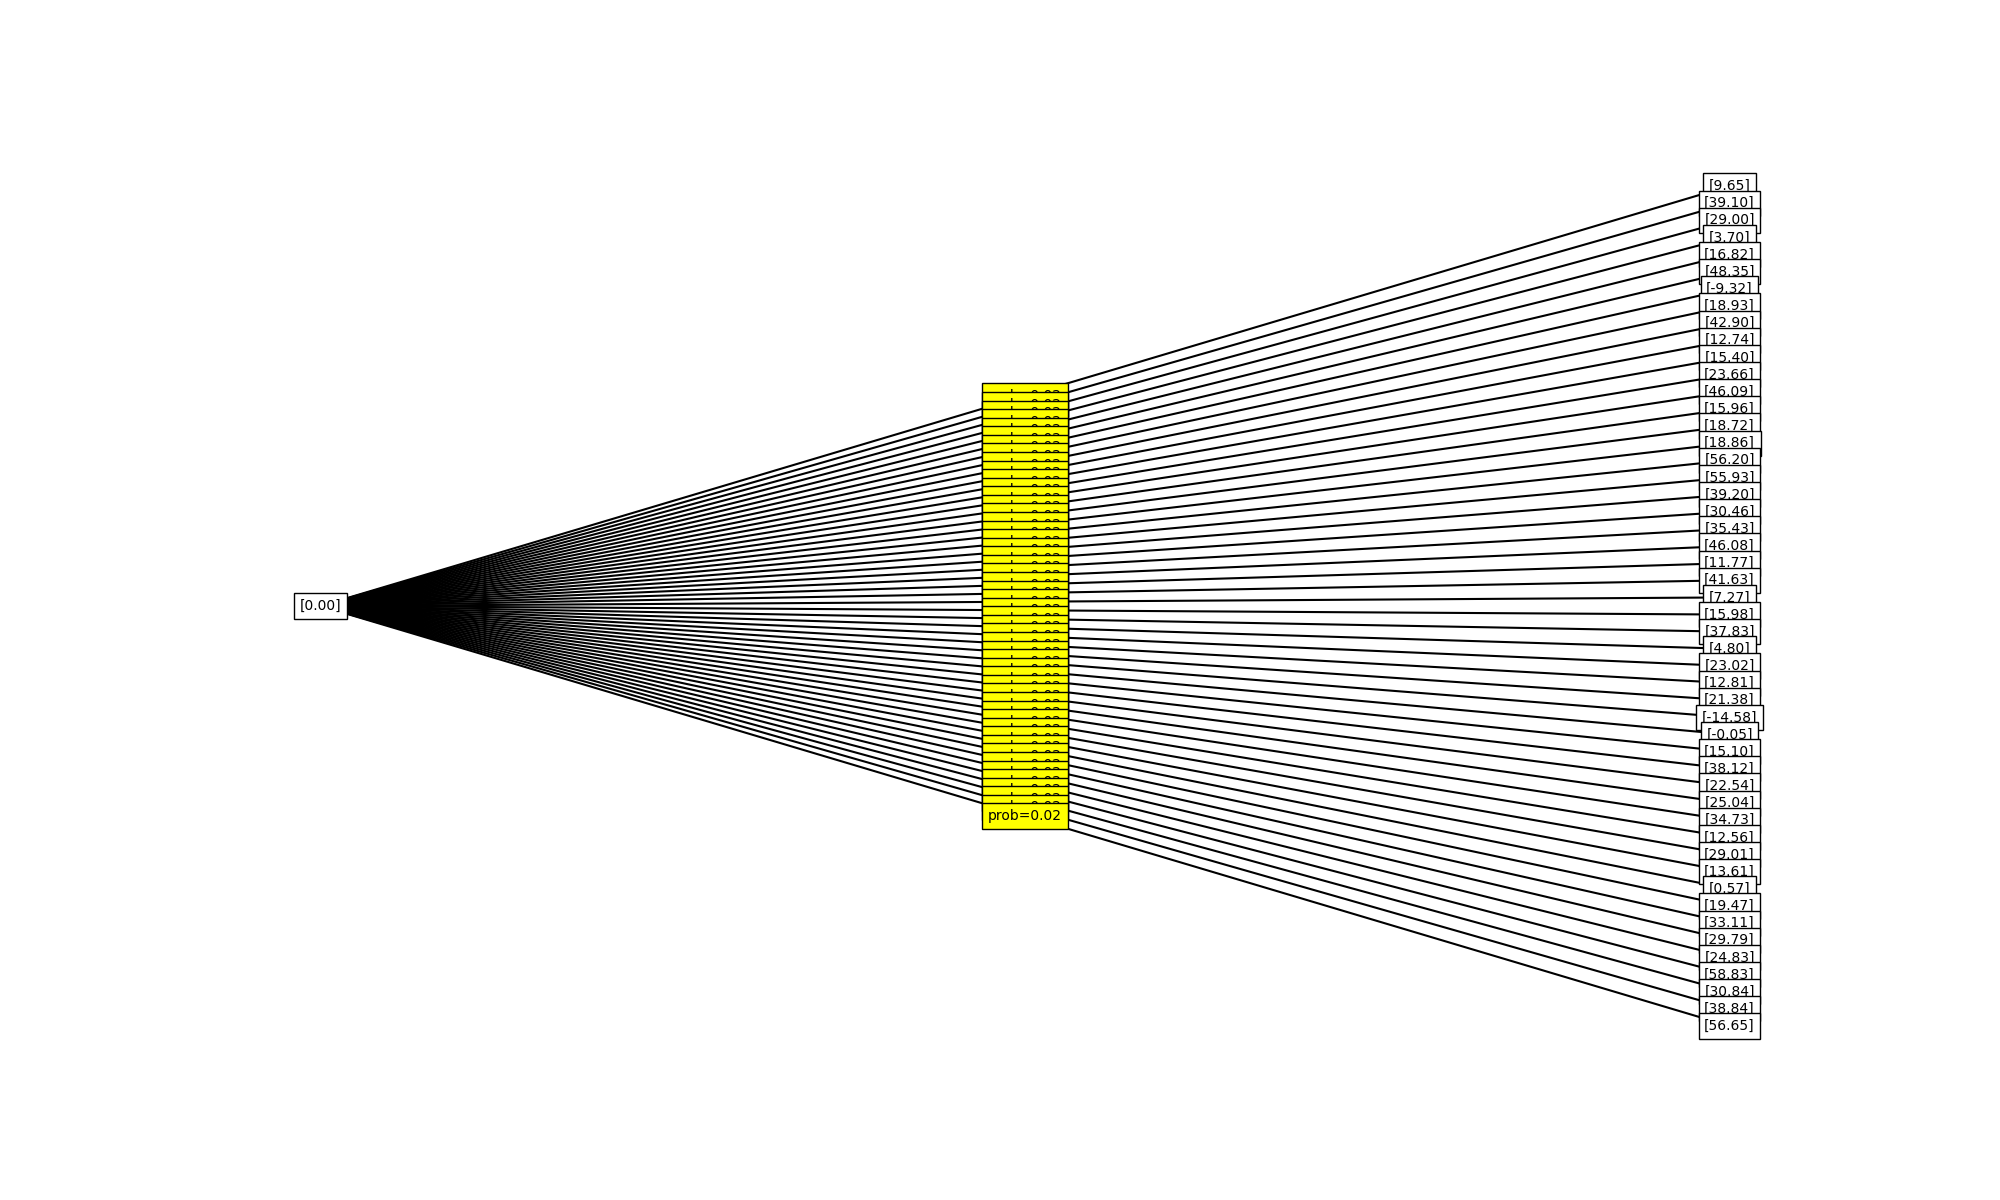
\includegraphics[width=1\textwidth]{../immagini/scenariNV.png}
		\caption{Visualization of an example of scenario tree, used in the analysis of the Newsvendor problem. The tree is composed of 10 equiprobabilistic sets, each of dimension 5 sampled from a multivariate normal distribution of dimension 5 with parameters $\mu = 25, \sigma^{2} = 200$, before rounding and aggregation. The scenario tree clearly illustrating the branching structure, node values, and probabilities. }
		\label{fig:scenariotree-plot}
	\end{figure}
	
	\noindent
	The following tables and statistical summaries present the main results obtained from the repeated solution of the Newsvendor problem using all generated and aggregated demand scenarios. These include the key descriptive statistics for the expected profit and the confidence intervals estimated over multiple simulation sets, i.e. :
	\begin{itemize}
		\item $\bar{p}_{N}:$ estimation of the expected value of the profit with $95\%$ confidence interval, obtained by considering the sample mean computed using the $N$ values from solving the problem for each sample; 
		\item $s^{2}_{N}:$ sample variance of the expected value of the profit,
	\end{itemize}
	
	\noindent where $N = 20,74.$
	
	\begin{table}[H]
		\centering
			\begin{tabular}{|c|c|c|}
			\hline
			\textbf{Number of Sets} & \textbf{Mean Profit (€)} & \textbf{Std. Deviation (€)} \\
			\hline
			20 & 198.62 & 21.99 \\
			74 & 204.12 & 17.30 \\
			\hline
		\end{tabular}
		\caption{Descriptive statistics of expected profit for Newsvendor simulation sets.}
		
		\label{tab:profit-descriptive}
	\end{table}
	
	\begin{table}[H]
		\centering
		\begin{tabular}{|c|c|c|}
			\hline
			\textbf{Number of Sets} & \textbf{95\% Confidence Interval (€)} & \textbf{Interval Width (€)} \\
			\hline
			20 & (188.98,\;208.26) & 19.27 \\
			74 & (200.18,\;208.07) & 7.88 \\
			\hline
		\end{tabular}
		\caption{Confidence intervals for expected profit for Newsvendor problem considering all samples generated.}
		
		\label{tab:profit-ci}
	\end{table}
	

	\subsection{ATO Problem}
	
	This subsection presents the results of the Assemble-to-Order (ATO) optimization model using the complete set of scenarios generated by our stochastic model.\\
	
	\noindent To analyze the problem, 85 samples of not necessarily equal cardinality, but from the same distribution, were generated to simulate the behavior of the random variable demand. The fact that not all samples have the same cardinality highlights the different types of demand that can occur; nevertheless scenarios were generated with a maximum cardinality, related to the use of a limited Gurobi license. Next, 85 ATO problems were solved, then as many samples of the expected value of profit were obtained. The 85 value was chosen so as to construct a $95\%$ confidence interval for the expected value of profit. \\
	
	\noindent The scenarios were generated as follows: 
	\begin{enumerate}
		\item Through the scenario tree class, from an initial fixed root, 85 nodes of size 80 were sampled; each set consists of the succession of 40 pairs [Item 1,Item 2], where each pair represents the realization of a possible demand scenario. They are sampled from the multivariate normal $\mathcal{N}_{2}(\mu, \Sigma)$ with $\mu = [10,16]$ and covariance matrix $\Sigma =  \begin{pmatrix} 70 &0  \\ 0 &90  \end{pmatrix} $.The choice of $\mu$ and $\Sigma$ parameters was dictated by the possibility of generating data that encapsulated some variability, produce results that could be reasonable and allow the problem to be solved even with a limited Gurobi license. 
		
		\item The scenario tree generated returns demand values as floating-point numbers. However, since the ATO problem inherently deals with discrete units (we are talking about number of pizzas), these continuous observations must be rounded to the nearest integer and constrained to be non-negative, ensuring practical and realistic demand scenarios. This rounding and aggregation procedure is implemented in the code using the provided \texttt{aggregate\_discrete\_demands} function, which combines scenarios with identical integer demands, summing their probabilities.
		
	\end{enumerate}
	
	\noindent In summary, also the ATO problem is solved 85 times for each generated set, which as a result of aggregation will be composed by a maximum number of realizations of demand scenarios equal to 40. Table (\ref{tab:ato-general-results}) shows an example of the output of a sample generated through the scenario tree, whose inputs were aggregated as necessary.
	%\newpage

	
	\begin{table}[H]
		\centering
		\footnotesize
		\label{tab:ato-general-results}
		\renewcommand{\arraystretch}{1.1}
		\begin{tabular}{|@{\hskip 2pt}p{3.2cm}@{\hskip 2pt}|@{\hskip 2pt}p{1cm}@{\hskip 2pt}||@{\hskip 2pt}p{3.2cm}@{\hskip 2pt}|@{\hskip 2pt}p{1cm}@{\hskip 2pt}||@{\hskip 2pt}p{3.2cm}@{\hskip 2pt}|@{\hskip 2pt}p{1cm}@{\hskip 2pt}|}
			\hline
			\textbf{Demand (Item 1, Item 2)} & \textbf{$\pi$} &
			\textbf{Demand (Item 1, Item 2)} & \textbf{$\pi$} &
			\textbf{Demand (Item 1, Item 2)} & \textbf{$\pi$} \\
			\hline
			\texttt{[0, 0]}    & 0.025 & \texttt{[4, 22]}   & 0.025 & \texttt{[13, 0]}   & 0.025 \\
			\texttt{[0, 1]}    & 0.025 & \texttt{[5, 4]}    & 0.025 & \texttt{[13, 12]}  & 0.025 \\
			\texttt{[0, 13]}   & 0.025 & \texttt{[6, 3]}    & 0.025 & \texttt{[14, 0]}   & 0.025 \\
			\texttt{[0, 21]}   & 0.025 & \texttt{[6, 10]}   & 0.050 & \texttt{[14, 4]}   & 0.025 \\
			\texttt{[0, 24]}   & 0.025 & \texttt{[7, 0]}    & 0.025 & \texttt{[14, 7]}   & 0.025 \\
			\texttt{[1, 2]}    & 0.025 & \texttt{[7, 10]}   & 0.025 & \texttt{[15, 7]}   & 0.025 \\
			\texttt{[1, 18]}   & 0.025 & \texttt{[8, 13]}   & 0.025 & \texttt{[15, 34]}  & 0.025 \\
			\texttt{[2, 18]}   & 0.025 & \texttt{[8, 14]}   & 0.025 & \texttt{[18, 14]}  & 0.025 \\
			\texttt{[3, 0]}    & 0.050 & \texttt{[9, 1]}    & 0.025 & \texttt{[18, 22]}  & 0.025 \\
			\texttt{[3, 13]}   & 0.025 & \texttt{[9, 4]}    & 0.025 & \texttt{[19, 8]}   & 0.025 \\
			\texttt{[3, 14]}   & 0.025 & \texttt{[11, 6]}   & 0.025 & \texttt{[20, 6]}   & 0.025 \\
			\texttt{[4, 6]}    & 0.025 & \texttt{[11, 20]}  & 0.025 & \texttt{[20, 12]}  & 0.025 \\
			\texttt{[22, 0]}   & 0.025 & \texttt{[13, 0]}   & 0.025 & \texttt{[21, 14]}  & 0.025 \\
			\hline
			\multicolumn{5}{|r|}{\textbf{Total}} & \textbf{1.00} \\
			\hline
		\end{tabular}
		\caption{An example of discrete demand values and aggregated probabilities used in the ATO model. First, an initial set with cardinality equal to 40 of equiprobabilistic scenarios (each scenario is a two-dimensional vector) was generated. Following the aggregation operation, the scenarios are reduced to 39, with probabilities no longer all equal.}
	\end{table}
	
	
	
	\newpage
	\noindent The plot in Figure~(\ref{fig:ato-scenariotree}) illustrating an example of scenario tree for an ATO problem  with the generated demand values, their probabilities, and the structure of uncertainty before aggregation.
	
	\begin{figure}[H]
		\centering
		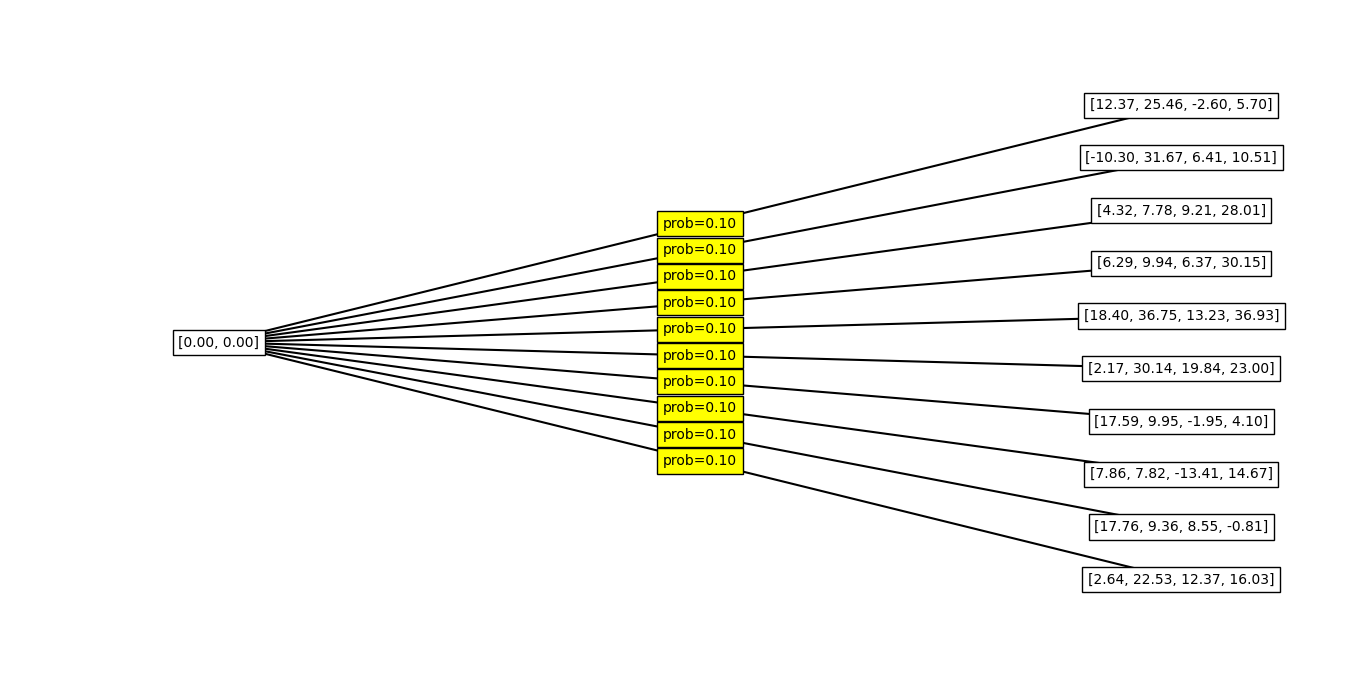
\includegraphics[width=1\textwidth]{../immagini/scenariATO.png}
		\caption{Visualization of an example of scenario tree, used in the analysis of the ATO problem. The tree is composed of 10 equiprobabilistic sets each of dimension 4, composed of two pairs [Item 1,Item 2], each sampled from a multivariate normal distribution of dimension 2 with parameters $\mu = [10,16], \Sigma = \begin{pmatrix} 70 &0  \\ 0 &90  \end{pmatrix}$ before rounding and aggregation.}
		\label{fig:ato-scenariotree}
	\end{figure}
	
	\noindent
	Table (\ref{tab:ATO-results-stat}) summarizes the main statistical indicators for the expected profit obtained from multiple independent simulation sets of the ATO problem, i.e.: 
	\begin{itemize}
		\item $\bar{p}_{N}:$ estimation of the expected value of the profit and $95\%$ confidence interval, obtained by considering the sample mean computed using the $N$ values from solving the problem for each sample; 
		\item $s^{2}_{N}:$ sample variance of the expected value of the profit,
	\end{itemize}
	
	\noindent where $N = 85, 20.$

	\[
	\begin{array}{cccc}
		\hline
		\text{Number of Sets} & \text{$\bar{p}_{N}$ (Mean Profit)} & \text{$s_{N}$ (Std. Dev.)} & \text{95\% Confidence Interval} \\
		\hline
		20 & 18.19 & 2.36 & (17.16,\; 19.23) \\
		85 & 18.79 & 2.14 & (18.34,\; 19.25) \\
		\hline
	\end{array}
	\]
	\label{tab:ATO-results-stat}
	
	
	\newpage
	\section{Results with K-means reduction}
	
	In this section, we present the results obtained by applying the K-means clustering method to reduce the number of scenarios and computational complexity generated in both the Newsvendor and Assemble-to-Order (ATO) problems.\\ 
	
	\noindent K-means is a clustering algorithm that, in our implementation, partitions the original set of scenarios into \(k\) clusters, by minimizing the weighted sum of squared distances between scenario values and their respective cluster centroids. Specifically, each original scenario is assigned to a cluster based on its proximity to the cluster's centroid, taking into account the scenario probabilities as weights. 
	%\newpage
	After the clustering process, the centroids become representative of the reduced scenarios, and the probabilities of these scenarios are recalculated by summing the probabilities of all original scenarios within each cluster.\\
	
	\noindent This procedure was implemented to reduce the number of original scenarios generated for both problems. The algorithm was applied to each of the N samples ($N = 74$ for Newsvendor, $N = 85$ for ATO), to reduce the numerosity of each sample to $k$, with $k \in [1,15]$. The upper bound of the interval was chosen such that the number of clusters obtained was significantly smaller than the original number of scenarios. Furthermore, for each of the N samples, the SSE trend graph was plotted to identify the appropriate number of points (clusters) to represent each initial set, according to the algorithm. The SSE is the sum of squared Euclidean distances of each point to its closest centroid, so is a measure of error.\\
	
	\noindent Below, we present detailed analyses of the performance of this scenario reduction method in the two considered optimization problems.
	\newpage
	\subsection{Newsvendor Problem}
	
	In order to analyze the Newsvendor problem with scenario reduction, $\forall k \in [1,15]$ and $N = 74$, the following were given in the table (\ref{tab:kmeans-nv-results}):
	\begin{itemize}
		\item $\bar{p}_{N}:$ estimation of the expected value of the profit with $95\%$ confidence interval, obtained by considering the sample mean computed using the $N$ values from solving the problem for each sample; 
		\item $sd_{N}:$ standard deviation of the expected value of the profit;
		\item $t_{R}:$ average computation time for reducing to $k$ scenarios;
		\item $t_{S}:$ average computation time for solving the Newsvendor problem with $k$ scenarios;
	\end{itemize}~
	\begin{table}[H]
		\[
		\begin{array}{ccccc}
			\hline
			\text{\# Cluster $(k)$} & \text{$\bar{p}_{N}$} & \text{$sd_{N}$} & \text{$t_{R}$ [s]} & \text{$t_{S}$ [s]} \\
			\hline
			1 & 227.92 & 17.45 & 0.0046 & 0.0004 \\
			2 & 214.71 & 18.27 & 0.0032 & 0.0005 \\
			3 & 210.94 & 17.77 & 0.0031 & 0.0004 \\
			4 & 207.22 & 17.30 & 0.0034 & 0.0005 \\
			5 & 206.25 & 17.52 & 0.0035 & 0.0006 \\
			6 & 205.94 & 17.61 & 0.0034 & 0.0005 \\
			7 & 205.45 & 17.23 & 0.0036 & 0.0006 \\
			8 & 204.84 & 17.41 & 0.0036 & 0.0006 \\
			9 & 204.73 & 17.37 & 0.0036 & 0.0006 \\
			10 & 204.56 & 17.47 & 0.0038 & 0.0007 \\
			11 & 204.40 & 17.51 & 0.0039 & 0.0007 \\
			12 & 204.49 & 17.49 & 0.0041 & 0.0008 \\
			13 & 204.39 & 17.48 & 0.0041 & 0.0008 \\
			14 & 204.32 & 17.52 & 0.0041 & 0.0009 \\
			15 & 204.23 & 17.52 & 0.0043 & 0.0010 \\
			\hline
		\end{array}
		\]
		\label{tab:kmeans-nv-results}
		\caption{Main results obtained from the repeated solution of the Newsvendor problem using $k$ scenarios (after reduction) with $k \in [1,15]$.}
	\end{table}
		
	
	\noindent These results demonstrate how scenario reduction via K-means effectively simplifies the scenario representation while preserving the essential characteristics needed to achieve reliable decision-making outcomes in stochastic optimization contexts.\\
	
	\noindent
	Additionally, Figure~\ref{fig:rendimentoK-nv} shows the trend of the sample mean expected profit as a function of the number of clusters $k$, including the corresponding standard deviation as error bars. This visualization highlights how increasing $k$ leads to more stable and less variable estimates of the expected profit, with the mean converging as $k$ grows.
	
	\begin{figure}[H]
		\centering
		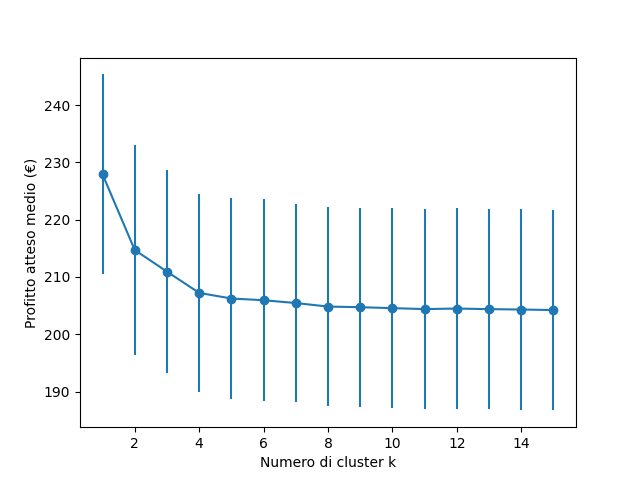
\includegraphics[width=0.7\textwidth]{../immagini/rendimentoK_nv.png}
		\caption{Sample mean of the expected profit and standard deviation as a function of the number of clusters $k$ for the Newsvendor problem.}
		\label{fig:rendimentoK-nv}
	\end{figure}
	
	
	\noindent The following is a plot of the trend in SSE for each sample as the number of $k$ scenarios to which each set is reduced varies. The figure shows that, following the kmeans algorithm, the appropriate number of points to which to reduce the numerosity of each set is around 3 and 4, depending on the sample.
	
	%\newpage
	\begin{figure}[H]
		\centering
		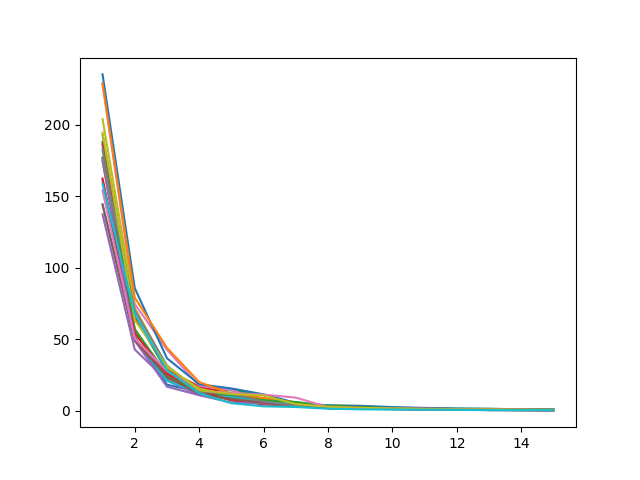
\includegraphics[width=0.8\textwidth]{../immagini/sseNV.png}
		\caption{SSE trend graph for $k \in [1,15]$ in case of Newsvendor problem. The figure shows that the appropriate number of points to which to reduce the numerosity of each set is around 3 and 4.}
		\label{fig:sse-nv}
	\end{figure}
	
	
	%\newpage
	\subsection{ATO Problem}
	In this subsection, we present the results obtained for the Assemble-to-Order (ATO) problem after applying scenario reduction via K-means clustering, to identify representative scenarios in a two-dimensional space (corresponding to the two final products). In order to analyze the newsvendor problem with scenario reduction, $\forall k \in [1,15]$ and $N = 85$ the following were given in the table (\ref{tab:kmeans-ato-results}):
	\begin{itemize}
		\item $\bar{p}_{N}:$ estimation of the expected value of the profit with $95\%$ confidence interval, obtained by considering the sample mean computed using the $N$ values from solving the problem for each sample; 
		\item $sd_{N}:$ standard deviation of the expected values of the profit;
		\item $t_{R}:$ average computation time for reducing to $k$ scenarios;
		\item $t_{S}:$ average computation time for solving the Newsvendor problem with $k$ scenarios;
	\end{itemize}~
	
	\begin{table}
		
	\[
	\begin{array}{ccccc}
		\hline
		\text{\# Cluster $(k)$} & \text{$\bar{p}_{N}$} & \text{$sd_{N}$} & \text{$t_{R}$\,[s]} & \text{$t_{S}$\,[s]} \\
		\hline
		1  & 24.00 & 0.00 & 0.0046 & 0.0014 \\
		2  & 23.82 & 0.83 & 0.0031 & 0.0015 \\
		3  & 22.38 & 3.06 & 0.0031 & 0.0016 \\
		4  & 20.15 & 5.02 & 0.0033 & 0.0017 \\
		5  & 18.60 & 5.27 & 0.0033 & 0.0018 \\
		6  & 18.25 & 4.69 & 0.0034 & 0.0018 \\
		7  & 17.68 & 4.58 & 0.0035 & 0.0020 \\
		8  & 18.02 & 4.09 & 0.0036 & 0.0020 \\
		9  & 17.56 & 3.76 & 0.0037 & 0.0022 \\
		10 & 17.54 & 3.63 & 0.0039 & 0.0023 \\
		11 & 17.61 & 3.34 & 0.0040 & 0.0024 \\
		12 & 17.62 & 3.38 & 0.0041 & 0.0025 \\
		13 & 17.50 & 3.45 & 0.0043 & 0.0026 \\
		14 & 17.53 & 3.50 & 0.0044 & 0.0027 \\
		15 & 17.43 & 3.43 & 0.0046 & 0.0028 \\
		\hline
	\end{array}
	\]
	\label{tab:kmeans-ato-results}
	\caption{Main results obtained from the repeated solution of the ATO problem using $k$ scenarios (after reduction) with $k \in [1,15]$.}
	\end{table}
	
	
	The scenario reduction via K-means preserved the essential characteristics of the demand distribution, allowing us to significantly reduce the problem size while maintaining optimality in the solution.	\\
	
	\noindent
	Additionally, Figure~(\ref{fig:rendimentoK-ato}) shows the trend of the sample mean expected profit as a function of the number of clusters $k$, including the corresponding standard deviation as error bars. This visualization highlights how increasing $k$ leads to more stable and less variable estimates of the expected profit, with the mean converging as $k$ grows.
	
	\begin{figure}[H]
		\centering
		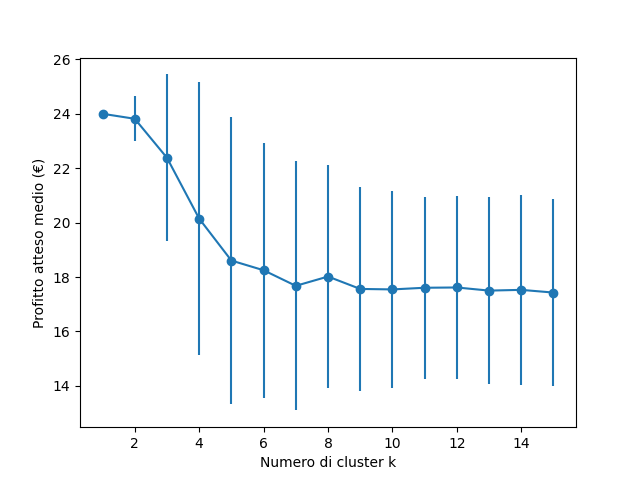
\includegraphics[width=0.7\textwidth]{../immagini/rendimentoK_ato.png}
		\caption{Sample mean of the expected profit and standard deviation as a function of the number of clusters $k$ for the Newsvendor problem.}
		\label{fig:rendimentoK-ato}
	\end{figure}
	
	\noindent The following is a plot of the trend in SSE for each sample as the number of $k$ scenarios to which each set is reduced varies. The figure shows that, following the kmeans algorithm, the appropriate number of points to which to reduce the numerosity of each set is around 3 and 4, depending on the sample.
	
	
	%\newpage
	\begin{figure}[H]
		\centering
		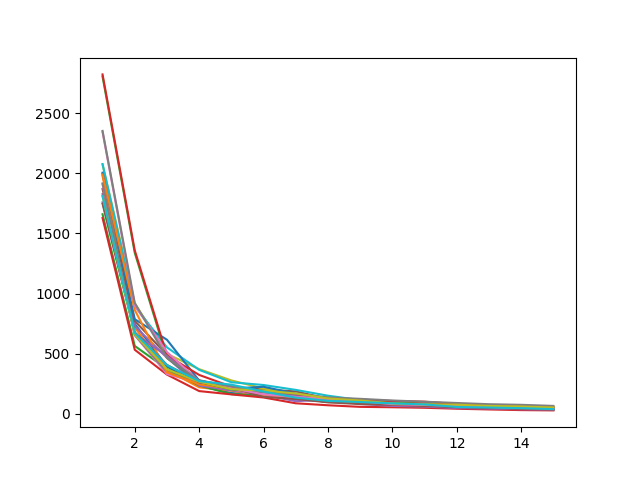
\includegraphics[width=0.8\textwidth]{../immagini/sseATO.png}
		\caption{SSE trend graph for $k \in [1,15]$ in case of ATO problem. The figure shows that the appropriate number of points to which to reduce the numerosity of each set is around 3 and 4.}
		\label{fig:sse-ato}
	\end{figure}
	
	\newpage
	\section{Results with Wasserstein distance--based reduction}
	
	In this section, we present the scenario reduction method based on the Wasserstein distance, as applied to both the Newsvendor and Assemble-to-Order (ATO) problems. The Wasserstein distance, also known as the Earth Mover's Distance, is a mathematical metric used to quantify the dissimilarity between two probability distributions on a given metric space. In the context of scenario reduction, it measures the minimum "cost" required to transform the original probability distribution of scenarios into a reduced one, where the "cost" is defined as the amount of probability mass to move times the distance it is moved.\\	
	
	\noindent Formally, let $\mu = (\mu_1, \ldots, \mu_m)$ and $\nu = (\nu_1, \ldots, \nu_n)$ be two discrete probability distributions on points ($x_1, \ldots, x_m$) and ($y_1, \ldots, y_n$). The $p$--Wasserstein distance is defined as:
	\[
	W_p(\mu, \nu) = \left( \min_{\gamma \in \Gamma(\mu, \nu)} \sum_{i=1}^m \sum_{j=1}^n \|x_i - y_j\|^p \gamma_{ij} \right)^{1/p}
	\]
	where $\gamma_{ij}$ is the transport plan representing the amount of mass moved from $x_i$ to $y_j$, and $\Gamma(\mu, \nu)$ is the set of admissible transport plans (satisfying mass conservation constraints). \\
	
	\noindent In our scenario reduction approach, we use an exact mixed-integer programming (MILP) formulation to select a subset of $k$ representative scenarios from the original $m$ scenarios, such that the Wasserstein distance between the original and reduced distributions is minimized. Below is reported the core optimization problem implemented in our code, in the unidimensional case:
	
	\[
	\begin{aligned}
		\min_{\gamma, z, \nu} \quad & \sum_{i=1}^m \sum_{j=1}^m c_{ij} \gamma_{ij} \\\\
		\text{s.t.} \quad
		& \sum_{j=1}^m \gamma_{ij} = \mu_i \qquad \forall i=1,\ldots,m \\
		& \sum_{i=1}^m \gamma_{ij} = \nu_j \qquad \forall j=1,\ldots,m \\
		& \nu_j \leq z_j \qquad \forall j=1,\ldots,m \\
		& \sum_{j=1}^m z_j = k \\
		& \sum_{j=1}^m \nu_j = 1 \\
		& z_j \in \{0,1\}, \quad \gamma_{ij}, \nu_j \geq 0
	\end{aligned}
	\]
	where:
	\begin{itemize}
		\item $c_{ij} = |x_i - x_j|^2$ is the cost of moving mass from scenario $i$ to scenario $j$ (Euclidean distance);
		\item $\gamma_{ij}$ is the amount of probability mass transported from $i$ to $j$;
		\item $z_j$ is a binary variable indicating whether scenario $j$ is selected in the reduced set;
		\item $\nu_j$ is the probability assigned to scenario $j$ in the reduced distribution.
	\end{itemize}
	\vspace{0.20cm}
	This model ensures that exactly $k$ scenarios are selected ($\sum_j z_j = k$), the reduced probabilities sum to 1, and the transportation of probability mass is minimized according to the cost matrix $C$. The same approach is extended to the multidimensional case (ATO problem), using the appropriate vector norms for the cost computation.
	The algorithm was applied to each of the 85 samples, to reduce the numerosity of each sample to $k$, with $k \in [1,15]$. Also for this problem, the upper bound of the interval was chosen such that the number of clusters obtained was significantly smaller than the original number of scenarios. \\
	
	\noindent Finally, it is important to point out that Wasserstein reduction technique, by construction, selects scenarios that preserve the probabilistic structure of the original distribution as faithfully as possible, yielding a reduced scenario set that guarantees a minimal loss of information with respect to the original distribution. In the following subsections, we detail the results obtained by applying this method to our stochastic optimization problems. 
	
	\subsection{Newsvendor Problem}
	
	For the Newsvendor problem, we applied the scenario reduction method based on the Wasserstein distance, which is designed to preserve the probabilistic structure of the original set of scenarios as closely as possible. The resulting reduced problems are summarized in Table~(\ref{tab:wass-nv-results}), where $\forall k \in [1,15]$ and $N = 74$ the following were given:
	\begin{itemize}
		\item $\bar{p}_{N}:$ estimation of the expected value of the profit with $95\%$ confidence interval, obtained by considering the sample mean computed using the $N$ values from solving the problem for each sample; 
		\item $sd_{N}:$ standard deviation of the expected values of the profit;
		\item $t_{R}:$ average computation time for reducing to $k$ scenarios;
		\item $t_{S}:$ average computation time for solving the Newsvendor problem with $k$ scenarios;
	\end{itemize}~
	
	\begin{table}[H]
	\[
	\begin{array}{ccccc}
		\hline
		\text{\# Cluster $(k)$} & \text{$\bar{p}_{N}$} & \text{$sd_{N}$} & \text{$t_{R}$\,[s]} & \text{$t_{S}$\,[s]} \\
		\hline
		1 & 228.41 & 17.86 & 0.0172 & 0.0003 \\
		2 & 216.11 & 17.63 & 0.2021 & 0.0005 \\
		3 & 209.96 & 17.69 & 0.2023 & 0.0005 \\
		4 & 206.41 & 17.82 & 0.1521 & 0.0005 \\
		5 & 205.84 & 17.75 & 0.1211 & 0.0006 \\
		6 & 205.17 & 17.50 & 0.1021 & 0.0006 \\
		7 & 205.12 & 17.29 & 0.0945 & 0.0007 \\
		8 & 204.61 & 17.26 & 0.0826 & 0.0007 \\
		9 & 204.57 & 17.40 & 0.0814 & 0.0007 \\
		10 & 204.48 & 17.34 & 0.0717 & 0.0007 \\
		11 & 204.41 & 17.46 & 0.0710 & 0.0008 \\
		12 & 204.41 & 17.50 & 0.0650 & 0.0009 \\
		13 & 204.37 & 17.47 & 0.0622 & 0.0011 \\
		14 & 204.24 & 17.43 & 0.0602 & 0.0012 \\
		15 & 204.32 & 17.57 & 0.0556 & 0.0012 \\
		\hline
	\end{array}
	\]
	\caption{Main results obtained from the repeated solution of the Newsvendor problem using $k$ scenarios (after reduction) with $k \in [1,15]$.}
	\label{tab:wass-nv-results}
	\end{table}
	
	\noindent These results demonstrate the effectiveness of Wasserstein reduction: although the number of scenarios is significantly decreased, the essential statistical features of the original demand distribution are maintained. The reduced scenario set still allows the optimization model to find a solution that is both robust and close to the original optimal profit.\\
	
	\noindent
	Additionally, Figure~(\ref{fig:rendimentoWass-nv}) shows the trend of the sample mean expected profit as a function of the number of clusters $k$, including the corresponding standard deviation as error bars. This visualization highlights how increasing $k$ leads to more stable and less variable estimates of the expected profit, with the mean converging as $k$ grows.
	
	\begin{figure}[H]
		\centering
		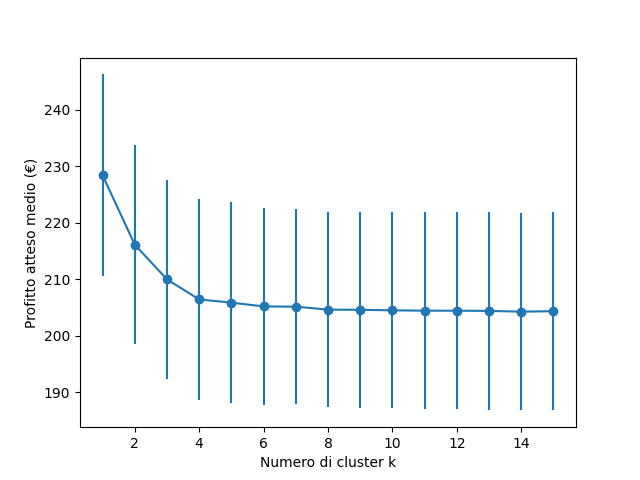
\includegraphics[width=0.7\textwidth]{../immagini/rendimentoWass_nv.png}
		\caption{Sample mean of the expected profit and standard deviation as a function of the number of clusters $k$ for the Newsvendor problem.}
		\label{fig:rendimentoWass-nv}
	\end{figure}	
	
	\subsection{ATO Problem}
	
	In this subsection, we report the results for the Assemble-to-Order (ATO) problem using scenario reduction via the Wasserstein distance. The original multidimensional demand scenarios were reduced to $k \in [1,15]$ representative scenarios by solving the exact MILP formulation that minimizes the Wasserstein distance, ensuring that the probabilistic and structural characteristics of the original distribution are preserved as faithfully as possible. The resulting reduced problems are summarized in Table(\ref{tab:wass-ato-results}), where $\forall k \in [1,15]$  and $N = 85 $ the following were given:
	\begin{itemize}
		\item $\bar{p}_{N}:$ estimation of the expected value of the profit with $95\%$ confidence interval, obtained by considering the sample mean computed using the $N$ values from solving the problem for each sample;
		\item $sd_{N}:$ sample variance of the expected values of the profit;
		\item $t_{R}:$ average computation time for reducing to $k$ scenarios;
		\item $t_{S}:$ average computation time for solving the Newsvendor problem with $k$ scenarios;
	\end{itemize}~
	
	\begin{table}[H]
	\[
	\begin{array}{ccccc}
		\hline
		\text{\# Cluster $(k)$} & \text{$\bar{p}_{N}$} & \text{$sd_{N}$} & \text{$t_{R}$\,[s]} & \text{$t_{S}$\,[s]} \\
		\hline
		1  & 23.94 & 0.24 & 0.0308 & 0.0016 \\
		2  & 23.37 & 0.97 & 0.4309 & 0.0019 \\
		3  & 22.58 & 1.32 & 0.3329 & 0.0021 \\
		4  & 21.78 & 2.09 & 0.2615 & 0.0023 \\
		5  & 21.11 & 2.26 & 0.2129 & 0.0025 \\
		6  & 20.67 & 2.48 & 0.1780 & 0.0026 \\
		7  & 20.12 & 2.39 & 0.1668 & 0.0027 \\
		8  & 19.82 & 2.49 & 0.1428 & 0.0028 \\
		9  & 19.67 & 2.42 & 0.1297 & 0.0029 \\
		10 & 19.52 & 2.38 & 0.1242 & 0.0029 \\
		11 & 19.39 & 2.40 & 0.1125 & 0.0029 \\
		12 & 19.24 & 2.32 & 0.1081 & 0.0030 \\
		13 & 19.16 & 2.32 & 0.1018 & 0.0031 \\
		14 & 19.00 & 2.35 & 0.0946 & 0.0032 \\
		15 & 18.96 & 2.28 & 0.0907 & 0.0034 \\
		\hline
	\end{array}
	\]
	\caption{Main results obtained from the repeated solution of the ATO problem using $k$ scenarios (after reduction) with $k \in [1,15]$.}
	\label{tab:wass-ato-results}
	\end{table}
	This outcome highlights the robustness and accuracy of the Wasserstein-based scenario reduction, which manages to preserve the key features of the stochastic demand while significantly reducing computational complexity.\\
	
	\noindent
	Additionally, Figure~(\ref{fig:rendimentoWass-ato}) shows the trend of the sample mean expected profit as a function of the number of clusters $k$, including the corresponding standard deviation as error bars. This visualization highlights how increasing $k$ leads to more stable and less variable estimates of the expected profit, with the mean converging as $k$ grows.
	
	\begin{figure}[H]
		\centering
		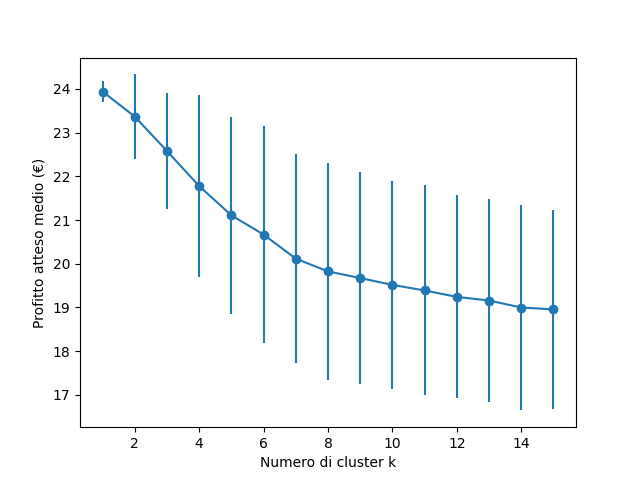
\includegraphics[width=0.7\textwidth]{../immagini/rendimentoWass_ato.png}
		\caption{Sample mean of the expected profit and standard deviation as a function of the number of clusters $k$ for the ATO problem.}
		\label{fig:rendimentoWass-ato}
	\end{figure}
	
	\newpage	
	\section{Efficiency}
	
	In this section, we analyze and compare the computational efficiency of the scenario reduction techniques for both the Newsvendor and ATO problems. The analysis focuses on the execution times of the full solution, the K-means clustering reduction, and the Wasserstein distance-based reduction for varying values of $k$. All times are averaged over the different samples for each case.\\
	
	\noindent Figure~(\ref{fig:timing-ato}) reports the total computation times for the ATO problem, including both the scenario reduction (with K-means and Wasserstein) and the subsequent optimization for $k \in [1,15]$. Each bar shows the average execution time for the corresponding algorithm and cluster size. It is evident that, while the time required for solving the reduced optimization problems remains almost negligible, the time spent in scenario reduction (especially using the Wasserstein approach) can become significant, and grows as $k$ decreases. The Wasserstein reduction is consistently more expensive than K-means, particularly for small $k$, due to the MILP formulation solved for each sample.
	
	\begin{figure}[H]
		\centering
		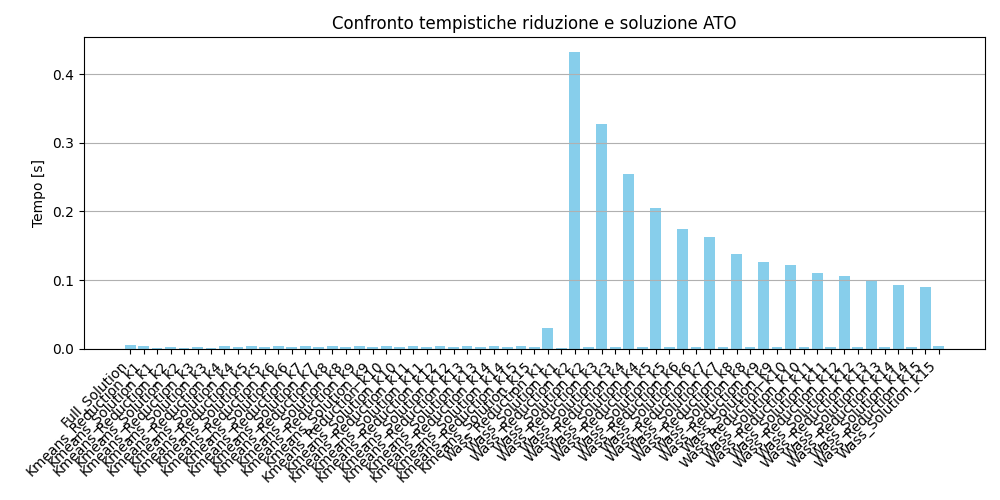
\includegraphics[width=1\textwidth]{../immagini/tempi_ato.png}
		\caption{Computation times for scenario reduction and solution phases for the ATO problem, as a function of the number of clusters $k$.}
		\label{fig:timing-ato}
	\end{figure}
	
	\vspace{0.5em}
	\noindent
	Overall, these results highlight a trade-off between the quality of the reduced scenario set and the computational effort required to obtain it. K-means offers fast reduction with reasonable accuracy, while Wasserstein provides higher-fidelity reduction at the cost of significantly longer computation times, particularly for multidimensional or large-sample problems.
	
	 \begin{figure}[H]
		     \centering
		     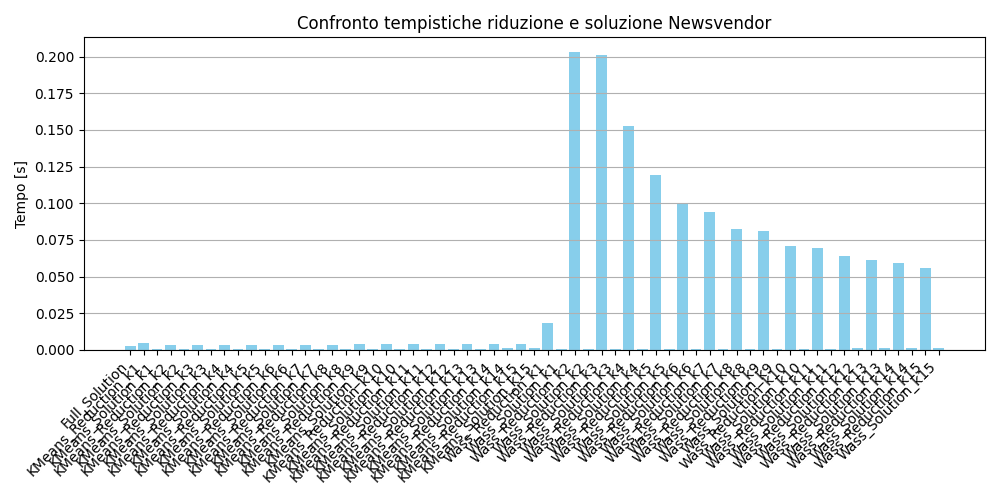
\includegraphics[width=1\textwidth]{../immagini/tempi_nv.png}
		     \caption{Computation times for scenario reduction and solution phases for the Newsvendor problem, as a function of the number of clusters $k$.}
		     \label{fig:timing-nv}
		 \end{figure}
	
	\noindent
	A direct comparison between the Newsvendor and ATO problems reveals that the same trends hold across both applications. As shown in Figure~(\ref{fig:timing-nv}) for the Newsvendor problem, the total execution time for scenario reduction using the Wasserstein approach is substantially higher than for K-means, especially for low values of $k$, confirming the computational burden of the MILP-based method. The optimization times themselves, for both problems, are consistently negligible compared to the reduction phases.	Notably, as the number of clusters $k$ increases, the computational gap between K-means and Wasserstein narrows, yet the latter always remains more expensive. This effect is even more pronounced in the ATO problem, where the multidimensional nature of the scenarios further increases the cost of Wasserstein reduction. \\
	
	\noindent These results emphasize the practical trade-off: while Wasserstein-based scenario reduction may yield a reduced set that better preserves the probabilistic features of the original distribution, the K-means heuristic is far more computationally efficient and, as observed in previous sections, delivers very similar performance in terms of solution quality for both studied problems. Thus, for large-scale or high-dimensional problems, K-means remains the preferred option unless maximum distributional fidelity is required.
	
	
	\newpage
	
	\section{Discussion}
	
	\noindent The analysis presented in this report highlight important aspects regarding both the quality of solutions and the computational efficiency of different scenario reduction techniques when applied to the Newsvendor and Assemble-to-Order (ATO) problems.\\
	
	\noindent From the chart, we observe that the time required to solve the full problem without reduction (\texttt{Full\_Solution}) is significantly lower than the time spent in the reduction phases (\texttt{KMeans\_Reduction} and \texttt{Wasserstein\_Reduction}), which dominate the total computational cost. Conversely, the actual optimization on the reduced scenario sets (\texttt{KMeans\_Solution} and 
	
	\texttt{Wasserstein\_Solution}) is almost negligible in terms of time. This result highlights that the bottleneck is the reduction procedure itself --especially when using methods such as K-means or Wasserstein MILP— while the optimization stage becomes extremely fast once the scenario set is reduced. Therefore, the choice of the reduction algorithm and its implementation has a direct impact on the overall computational efficiency of the workflow. However, once the reduced scenario set is obtained, the final optimization becomes extremely efficient. This analysis confirms that, for moderate instance sizes, the major computational effort is concentrated in the scenario reduction phase—especially for methods based on mathematical programming—while the actual optimization benefits greatly from working on a smaller scenario set. Thus, efficiency considerations must take into account not only the quality of the reduced scenarios, but also the time required for the reduction procedure itself. \\
	
	
\noindent	From a solution perspective, all scenario reduction methods—K-means and Wasserstein distance—were able to preserve the essential structure of the original problems, although, by its nature, heuristics based on Wasserstein distance are able to remain more faithful to the probabilistic information contained in the initial data. In both cases, the expected profits derived from the reduced sets of scenarios have a decreasing trend as $k$ increases, and tends to get closer to those derived from the full set of scenarios. A reduction that does not require too large a number of new clusters (note that for both problems the maximum value of $k$ was set at 15), keeps the expected value results fairly close to those obtained through the starting set of scenarios. However, it is worth mentioning that, in reducing the scenarios through Kmeans, the standard deviation of the obtained estimate is larger than the case in which the full set of scenarios are considered. In contrast, for the reduction of scenarios based on Wasserstein distance, the standard deviation is smaller when compared with that associated with the “rival” reduction technique, and more faithful to that obtained in the case where the full set of scenarios are considered. This was exactly what was expected from the nature of this heuristics, which despite the computational cost, tend to better preserve and capture the probabilistic information present in the original samples. Moreover, looking at the SSE graphs, for both problems clustering through Kmeans suggests that values such as 3-4 are sufficient to have a fairly accurate description of the source problem. Comparing this with the values obtained, it can be observed that, in our study, this is true for the Newsvendor problem, but false for the ATO problem, probably due to its more complex nature. For this problem, in fact, for $k = 4$ the expected value estimate is still quite far from a solution that is satisfactory enough.\\
	
	\noindent In conclusion, the choice of the reduction technique may be guided by the available computational resources and the problem's dimensionality: K-means offers faster execution and satisfactory accuracy for most practical purposes, while the Wasserstein approach is preferable when maximum fidelity to the original probability distribution is required, at the expense of increased computation time.
	
	%	\begin{table}[htbp]
		%		\centering
		%		\caption{Summary of optimal solutions and objective values for both Newsvendor and ATO problems.}
		%		\begin{tabular}{|l|l|c|c|c|}
			%			\hline
			%			\textbf{Problem} & \textbf{Method} & \textbf{\# Scenarios} & \textbf{Optimal Variable} & \textbf{Objective Value (€)} \\
			%			\hline
			%			Newsvendor & Full           & 31 & $x^* = 48$          & 202.00 \\
			%			Newsvendor & K-means        & 5  & $x^* = 45$          & 201.20 \\
			%			Newsvendor & Wasserstein    & 5  & $x^* = 42$          & 203.60 \\
			%			\hline
			%			ATO        & Full           & 36 & $x^* = [8,\,8,\,0]$ & 32.00  \\
			%			ATO        & K-means        & 5  & $x^* = [8,\,8,\,0]$ & 32.00  \\
			%			ATO        & Wasserstein    & 5  & $x^* = [8,\,8,\,0]$ & 32.00  \\
			%			\hline
			%		\end{tabular}
		%		\label{tab:summary-results}
		%	\end{table}

\appendix
\section{Appendix: Python Codes}	
\addcontentsline{toc}{section}{Appendix: Python Codes}



\subsection{scenarioTree.py}
\addcontentsline{toc}{subsection}{scenarioTree.py}
\noindent The following file illustrates the Scenario Tree class, containing both methods for generating scenario trees (to be used to analyze the required problems) and for reducing them.

\definecolor{darkred}{rgb}{0.6,0.0,0.0}
\definecolor{darkgreen}{rgb}{0,0.50,0}
\definecolor{lightblue}{rgb}{0.0,0.42,0.91}
\definecolor{orange}{rgb}{0.99,0.48,0.13}
\definecolor{grass}{rgb}{0.18,0.80,0.18}
\definecolor{pink}{rgb}{0.97,0.15,0.45}


% General Setting of listings
%\lstset{
%	aboveskip=1em,
%	breaklines=true,
%	abovecaptionskip=-6pt,
%	captionpos=b,
%	escapeinside={\%*}{*)},
%	frame=single,
%	numbers=left,
%	numbersep=15pt,
%	numberstyle=\tiny,
%}

% 1. General Python Keywords List
\lstdefinelanguage{PythonPlus}[]{Python}{
	morekeywords=[1]{,as,assert,nonlocal,with,yield,self,True,False,None,} % Python builtin
	morekeywords=[2]{,__init__,__add__,__mul__,__div__,__sub__,__call__,__getitem__,__setitem__,__eq__,__ne__,__nonzero__,__rmul__,__radd__,__repr__,__str__,__get__,__truediv__,__pow__,__name__,__future__,__all__,}, % magic methods
	morekeywords=[3]{,object,type,isinstance,copy,deepcopy,zip,enumerate,reversed,list,set,len,dict,tuple,range,xrange,append,execfile,real,imag,reduce,str,repr,}, % common functions
	morekeywords=[4]{,Exception,NameError,IndexError,SyntaxError,TypeError,ValueError,OverflowError,ZeroDivisionError,}, % errors
	morekeywords=[5]{,ode,fsolve,sqrt,exp,sin,cos,arctan,arctan2,arccos,pi, array,norm,solve,dot,arange,isscalar,max,sum,flatten,shape,reshape,find,any,all,abs,plot,linspace,legend,quad,polyval,polyfit,hstack,concatenate,vstack,column_stack,empty,zeros,ones,rand,vander,grid,pcolor,eig,eigs,eigvals,svd,qr,tan,det,logspace,roll,min,mean,cumsum,cumprod,diff,vectorize,lstsq,cla,eye,xlabel,ylabel,squeeze,}, % numpy / math
}

% 3. Extended theme
\lstdefinestyle{colorEX}{
	basicstyle=\ttfamily,
	backgroundcolor=\color{white},
	commentstyle=\color{darkgreen}\slshape,
	keywordstyle=\color{blue}\bfseries\itshape,
	keywordstyle=[2]\color{blue}\bfseries,
	keywordstyle=[3]\color{grass},
	keywordstyle=[4]\color{red},
	keywordstyle=[5]\color{orange},
	stringstyle=\color{darkred},
	emphstyle=\color{pink}\underbar,
	showspaces=false, % Do not show spaces
	showstringspaces=false, % Do not show spaces in strings
%	frame=single, % Single-line frame
	aboveskip=1em,
	breaklines=true,
%	abovecaptionskip=-6pt,
	captionpos=b,
	escapeinside={\%*}{*)},
	frame=single,
	numbers=left,
	numbersep=15pt,
	numberstyle=\tiny,
	}

\lstset{style=colorEX}
%\lstinputlisting[language=python,caption={class Scenario\_Tree},label={lst:scenariotree}]{/home/simona/Documenti/NO4LSP-SO-project/Stocasthic_optimization/codici/scenario_tree/scenarioTree.py}
\begin{lstlisting}[language=python,caption={class ScenarioTree},label={lst:class-scenario-tree}]
# -*- coding: utf-8 -*-
import os
import time
import logging
import numpy as np
import networkx as nx
import matplotlib.pyplot as plt
from .stochModel import StochModel
from sklearn.cluster import KMeans
import gurobipy as gp
from gurobipy import GRB
from collections import defaultdict


setseed = 42

class ScenarioTree(nx.DiGraph):
def __init__(self, name: str, branching_factors: list, len_vector: int, initial_value, stoch_model: StochModel):
nx.DiGraph.__init__(self)
starttimer = time.time()
self.starting_node = 0
self.len_vector = len_vector # number of stochastic variables
self.stoch_model = stoch_model # stochastic model used to generate the tree
depth = len(branching_factors) # tree depth
self.add_node( # add the node 0  
self.starting_node,
obs=initial_value,
prob=1,
id=0,
stage=0,
remaining_times=depth,
path_prob=1 # path probability from the root node to the current node
)    
self.name = name
self.filtration = []
self.branching_factors = branching_factors
self.n_scenarios = np.prod(self.branching_factors)
self.nodes_time = []
self.nodes_time.append([self.starting_node])

# Build the tree
count = 1
last_added_nodes = [self.starting_node]
# Main loop: until the time horizon is reached
for i in range(depth):
next_level = []
self.nodes_time.append([])
self.filtration.append([])

# For each node of the last generated period add its children through the StochModel class
for parent_node in last_added_nodes:
# Probabilities and observations are given by the stochastic model chosen
p, x = self._generate_one_time_step(self.branching_factors[i], self.nodes[parent_node])
# Add all the generated nodes to the tree
for j in range(self.branching_factors[i]):
id_new_node = count
self.add_node(
id_new_node,
obs=x[:,j],
prob=p[j],
id=count,
stage=i+1,
remaining_times=depth-1-i,
path_prob=p[j]*self._node[parent_node]['path_prob'] # path probability from the root node to the current node
)
self.add_edge(parent_node, id_new_node)
next_level.append(id_new_node)
self.nodes_time[-1].append(id_new_node)
count += 1
last_added_nodes = next_level
self.n_nodes = count
self.leaves = last_added_nodes

endtimer = time.time()
logging.info(f"Computational time to generate the entire tree:{endtimer-starttimer} seconds")

# Method to plot the tree
def plot(self, file_path=None):
_, ax = plt.subplots(figsize=(20, 12))
x = np.zeros(self.n_nodes)
y = np.zeros(self.n_nodes)
x_spacing = 15
y_spacing = 200000
for time in self.nodes_time:
for node in time:
obs_str = ', '.join([f"{ele:.2f}" for ele in self.nodes[node]['obs']])
ax.text(
x[node], y[node], f"[{obs_str}]", 
ha='center', va='center', bbox=dict(
facecolor='white',
edgecolor='black'
)
)
children = [child for parent, child in self.edges if parent == node]
if len(children) % 2 == 0:
iter = 1
for child in children:
x[child] = x[node] + x_spacing
y[child] = y[node] + y_spacing * (0.5 * len(children) - iter) + 0.5 * y_spacing
ax.plot([x[node], x[child]], [y[node], y[child]], '-k')
prob = self.nodes[child]['prob']
ax.text(
(x[node] + x[child]) / 2, (y[node] + y[child]) / 2,
f"prob={prob:.2f}",
ha='center', va='center',
bbox=dict(facecolor='yellow', edgecolor='black')
)                        
iter += 1

else:
iter = 0
for child in children:
x[child] = x[node] + x_spacing
y[child] = y[node] + y_spacing * ((len(children)//2) - iter)
ax.plot([x[node], x[child]], [y[node], y[child]], '-k')
prob = self.nodes[child]['prob']
ax.text(
(x[node] + x[child]) / 2, (y[node] + y[child]) / 2,
f"prob={prob:.2f}",
ha='center', va='center',
bbox=dict(facecolor='yellow', edgecolor='black')
)                        
iter += 1
y_spacing = y_spacing * 0.25

#plt.title(self.name)
plt.axis('off')
if file_path:
plt.savefig(file_path)
plt.close()
else:
plt.show()


def _generate_one_time_step(self, n_scenarios, parent_node): 
'''Given a parent node and the number of children to generate, it returns the 
children with corresponding probabilities'''
prob, obs = self.stoch_model.simulate_one_time_step(
parent_node=parent_node,
n_children=n_scenarios
)
return prob, obs

#  ------------------------------------------------

def reduce_scenarios_kmeans_1D(self, X, mu, k, random_state=42):
"""
Reduces a discrete 1D distribution using weighted KMeans clustering.

Args:
X: array of shape (N,) - original scenario values (e.g., demand)
mu: array of shape (N,) - associated probabilities (sum = 1)
k: int - desired number of reduced scenarios
random_state: int - for reproducibility

Returns:
centers_sorted: list of the new (sorted) scenario values
probs_sorted: list of the new (sorted) associated probabilities
"""        

X = np.asarray(X).reshape(-1, 1)
mu = np.asarray(mu)


# 1) Clustering KMeans pesato
kmeans = KMeans(n_clusters=k, random_state=random_state)
kmeans.fit(X, sample_weight=mu)
sse_kj = kmeans.inertia_

centers = kmeans.cluster_centers_.flatten()
labels = kmeans.labels_

# 2) nuove probabilita' come somma dei pesi in ciascun cluster
probs = np.zeros(k)
for i in range(len(X)):
probs[labels[i]] += mu[i]

# 3) Arrotonda e ordina per valore crescente della domanda
pairs = sorted(zip(centers, probs), key=lambda x: x[0])
centers_sorted = [round(float(c)) for c, _ in pairs]
probs_sorted   = [round(float(p), 4) for _, p in pairs]


return centers_sorted, probs_sorted, sse_kj

def reduce_scenarios_kmeans_multiD(self, X, mu, k, random_state=42):
"""
Reduces a discrete multi-dimensional distribution (e.g., for ATO) using weighted KMeans clustering.

Args:
X: array of shape (N, d) - original scenarios (e.g., [d1, d2])
mu: array of shape (N,) - associated probabilities (sum = 1)
k: int - desired number of reduced scenarios
random_state: int - for reproducibility

Returns:
centers_sorted: list of new scenarios (sorted by d1, d2)
probs_sorted: list of the new associated probabilities
"""

X = np.asarray(X)
mu = np.asarray(mu)

# Clustering KMeans pesato
kmeans = KMeans(n_clusters=k, random_state=random_state)
kmeans.fit(X, sample_weight=mu)
sse_kj = kmeans.inertia_

centers = kmeans.cluster_centers_
labels = kmeans.labels_

# nuove probabilita'
probs = np.zeros(k)
for i in range(len(X)):
probs[labels[i]] += mu[i]

# Arrotonda e ordina i risultati per (d1, d2)
centers_rounded = [
[int(round(c[0] / 10) * 10), int(round(c[1] / 10) * 10)]
for c in centers
]
probs_rounded   = [round(float(p), 4) for p in probs]

sorted_pairs = sorted(zip(centers_rounded, probs_rounded), key=lambda x: (x[0][0], x[0][1]))
centers_sorted, probs_sorted = zip(*sorted_pairs)

return list(centers_sorted), list(probs_sorted),sse_kj

#  ------------------------------------------------

def reduce_scenarios_wasserstein_1D(self, X, mu, k, p=2,
time_limit=None, verbose=False):
"""
Exact selection of k scenarios that minimize the Wasserstein distance (1-D).

Parameters
----------
X          : array-like, shape (m,)   original demand points
mu         : array-like, shape (m,)   original probabilities (sum = 1)
k          : int                      number of scenarios to keep
p          : int/float, default 1     L^p norm
time_limit : int/float or None        time limit in seconds for Gurobi
verbose    : bool                     if True, prints solver log

Returns
-------
Y_sorted   : list[int]     values of the selected k scenarios
nu_sorted  : list[float]   their probabilities (sum = 1)
"""

X  = np.asarray(X,  dtype=float).flatten()
mu = np.asarray(mu, dtype=float)
m  = len(X)
if k >= m:
raise ValueError("k deve essere < m")

# 1) matrice costi |xi - xj|^p
C = self.compute_cost_matrix_unidimensional(X, X, p=p)

# 2) modello 
mdl = gp.Model("ScenarioReductionMIP")
if not verbose:
mdl.setParam("OutputFlag", 0)
if time_limit:
mdl.setParam("TimeLimit", time_limit)

# variabili
gamma = mdl.addVars(m, m, lb=0.0, name="gamma")          # continui
z     = mdl.addVars(m, vtype=GRB.BINARY, name="z")       # binari
nu    = mdl.addVars(m, lb=0.0, name="nu")                # continui

# 3) obiettivo
mdl.setObjective(gp.quicksum(C[i, j] * gamma[i, j]
for i in range(m) for j in range(m)),
GRB.MINIMIZE)

# 4) vincoli supply: Sigma_j gamma_ij = mu_i
for i in range(m):
mdl.addConstr(gp.quicksum(gamma[i, j] for j in range(m)) == mu[i],
name=f"supply_{i}")

# 5) vincoli demand: Sigma_i gamma_ij = nu_j
for j in range(m):
mdl.addConstr(gp.quicksum(gamma[i, j] for i in range(m)) == nu[j],
name=f"demand_{j}")

# 6) supporto: nu_j <= z_j
for j in range(m):
mdl.addConstr(nu[j] <= z[j], name=f"support_{j}")

# 7) esattamente k scenari scelti
mdl.addConstr(gp.quicksum(z[j] for j in range(m)) == k, name="cardinality")

# 8) probabilita' totali = 1
mdl.addConstr(gp.quicksum(nu[j] for j in range(m)) == 1.0, name="sum_prob")

# 9) solve
mdl.optimize()

if mdl.status != GRB.OPTIMAL:
raise RuntimeError("Gurobi non ha trovato ottimo (stato %s)" % mdl.Status)

# 10) estrai risultati
sel_idx = [j for j in range(m) if z[j].X > 0.5]
Y       = X[sel_idx].astype(int)
nu_vals = np.array([nu[j].X for j in sel_idx])

# ordina
order = np.argsort(Y)
Y_sorted  = Y[order].tolist()
nu_sorted = [round(float(pv), 4) for pv in nu_vals[order]]

return Y_sorted, nu_sorted

def reduce_scenarios_wasserstein_multiD(self, X, mu, k, p=2,
time_limit=None, verbose=False):
"""
Exact selection of k scenarios (multi-D) that minimize the Wasserstein p-norm distance via MILP (Gurobi).

Parameters
----------
X          : array-like, shape (m, d)   original demand vectors
mu         : array-like, shape (m,)     original probabilities (sum = 1)
k          : int                        number of scenarios to retain
p          : int/float, default 2       L^p norm (2 = Euclidean)
time_limit : int/float or None          time limit in seconds for Gurobi
verbose    : bool                       True -> print solver log

Returns
-------
Y_sorted   : list[list[int]]   selected scenario vectors (sorted)
nu_sorted  : list[float]       corresponding probabilities (sum = 1)
"""

X  = np.asarray(X,  dtype=float)
mu = np.asarray(mu, dtype=float).flatten()
m, d = X.shape
if k >= m:
raise ValueError("k deve essere < numero scenari originali (m)")

# 1) matrice costi ||x_i - x_j||_p^p
C = self.compute_cost_matrix_multidimensional(X, X, p=p)      # shape (m, m)

# 2) modello 
mdl = gp.Model("ScenarioReductionMIP_multiD")
if not verbose:
mdl.setParam("OutputFlag", 0)
if time_limit:
mdl.setParam("TimeLimit", time_limit)

gamma = mdl.addVars(m, m, lb=0.0, name="gamma")           # continue
z     = mdl.addVars(m, vtype=GRB.BINARY, name="z")        # binarie
nu_v  = mdl.addVars(m, lb=0.0, name="nu")                 # continue

# 3) obiettivo
mdl.setObjective(
gp.quicksum(C[i, j]*gamma[i, j] for i in range(m) for j in range(m)),
GRB.MINIMIZE)

# 4) supply  Sigma_j gamma_ij = nu_i
for i in range(m):
mdl.addConstr(gp.quicksum(gamma[i, j] for j in range(m)) == mu[i],
name=f"supply_{i}")

# 5) demand  Sigma_i gamma_ij = nu_j
for j in range(m):
mdl.addConstr(gp.quicksum(gamma[i, j] for i in range(m)) == nu_v[j],
name=f"demand_{j}")

# 6) linking  nu_j <= z_j
for j in range(m):
mdl.addConstr(nu_v[j] <= z[j], name=f"support_{j}")

# 7) cardinalita': esattamente k scenari
mdl.addConstr(gp.quicksum(z[j] for j in range(m)) == k, name="cardinality")

# 8) probabilita' totali = 1
mdl.addConstr(gp.quicksum(nu_v[j] for j in range(m)) == 1.0, name="sum_prob")

# 9) solve
mdl.optimize()
if mdl.status != GRB.OPTIMAL:
raise RuntimeError(f"Gurobi status: {mdl.Status} (non ottimale)")

# 10) estrai scenari scelti e loro masse
sel_idx  = [j for j in range(m) if z[j].X > 0.5]
Y_sel    = X[sel_idx]                    # shape (k, d)
nu_sel   = np.array([nu_v[j].X for j in sel_idx])

# 11) ordina per comodita' (prima coord 0, poi 1, ...)
order    = np.lexsort(Y_sel.T[::-1])     # ordina per colonne crescenti
Y_sorted = Y_sel[order].round().astype(int).tolist()
nu_sorted= [round(float(nu_sel[t]), 4) for t in order]

return Y_sorted, nu_sorted

#  ------------------------------------------------

def compute_cost_matrix_multidimensional(self, points_mu, points_nu, p=2):
"""
Computes the cost matrix for multidimensional distributions.

Args:
points_mu: array of shape (m, d)
points_nu: array of shape (n, d)
p: norm to use (default = 2 for Euclidean distance)

Returns:
cost_matrix: array of shape (m, n)
"""

m = len(points_mu)
n = len(points_nu)

cost_matrix = np.zeros((m, n))

for i in range(m):
for j in range(n):
cost_matrix[i, j] = np.linalg.norm(np.array(np.array(points_mu[i]) - np.array(points_nu[j])), ord=p)
return cost_matrix

#############################################
def compute_cost_matrix_unidimensional(self, points_mu, points_nu, p=2):
"""
Compute the cost matrix using a given p-norm.

Parameters:
-----------
points_mu : array-like, shape (m, d)
Coordinates of points corresponding to the distribution mu (source points).
points_nu : array-like, shape (n, d)
Coordinates of points corresponding to the distribution nu (target points).
p : float, optional (default=2)
The p-norm to use for computing the cost (e.g., p=2 for Euclidean distance, p=1 for Manhattan distance).

Returns:
--------
cost_matrix : array, shape (m, n)
The cost matrix where cost_matrix[i, j] is the distance (cost) between points_mu[i] and points_nu[j].
"""
m = len(points_mu)
n = len(points_nu)

cost_matrix = np.zeros((m, n))

for i in range(m):
for j in range(n):
# Compute the p-norm distance between point i in mu and point j in nu
cost_matrix[i, j] = abs(points_mu[i] - points_nu[j])**p
return cost_matrix

#############################################

def wasserstein_distance(self, mu, nu, cost_matrix):
"""
Compute the 1-Wasserstein distance between two discrete distributions using Gurobi.

Parameters:
-----------
mu : array-like, shape (m,)
Probability distribution of the first set of points (source).
nu : array-like, shape (n,)
Probability distribution of the second set of points (target).
cost_matrix : array-like, shape (m, n)
The cost matrix where cost_matrix[i][j] is the cost of transporting mass from
point i in mu to point j in nu.

Returns:
--------
wasserstein_distance : float
The computed Wasserstein distance between mu and nu.
transport_plan : array, shape (m, n)
The optimal transport plan.
"""
m = len(mu)
n = len(nu)

# Create a Gurobi model
model = gp.Model("wasserstein")

# Disable Gurobi output 
model.setParam("OutputFlag", 0)

# Decision variables: transport plan gamma_ij
gamma = model.addVars(m, n, lb=0, ub=GRB.INFINITY, name="gamma")

# Objective: minimize the sum of the transport costs
model.setObjective(gp.quicksum(cost_matrix[i, j] * gamma[i, j] for i in range(m) for j in range(n)), GRB.MINIMIZE)

# Constraints: ensure that the total mass transported from each mu_i matches the corresponding mass in mu
for i in range(m):
model.addConstr(gp.quicksum(gamma[i, j] for j in range(n)) == mu[i], name=f"supply_{i}")

# Constraints: ensure that the total mass transported to each nu_j matches the corresponding mass in nu
for j in range(n):
model.addConstr(gp.quicksum(gamma[i, j] for i in range(m)) == nu[j], name=f"demand_{j}")

# Solve the optimization model
model.optimize()

# Extract the optimal transport plan and the Wasserstein distance
if model.status == GRB.OPTIMAL:
transport_plan = np.zeros((m, n))
for i in range(m):
for j in range(n):
transport_plan[i, j] = gamma[i, j].X
wasserstein_distance = model.objVal
return wasserstein_distance, transport_plan
else:
raise Exception("Optimization problem did not converge!")

#############################################

def aggregate_discrete_demands(self, demands, probs, round_probs=2):
"""
Aggregates and sorts discrete scenarios by summing the probabilities associated with identical demand values.

Args:
demands: list of integer demand values
probs: list of corresponding probabilities
round_probs: number of decimal digits to round the final probabilities

Returns:
(demands_agg, probs_agg): parallel lists, sorted in increasing order
"""

demand_prob = defaultdict(float)
for d, p in zip(demands, probs):
demand_prob[d] += p

# Ordina per chiave (domanda crescente)
items = sorted(demand_prob.items())

demands_agg = [d for d, _ in items]
probs_agg = [round(p, round_probs) for _, p in items]

return demands_agg, probs_agg

#############################################

def aggregate_vectorial_demands(self, demand_vectors, probs, round_probs=3):
"""
Aggregates vectorial scenarios by summing the probabilities associated with identical demand vectors,

Args:
demand_vectors: list of lists or tuples (e.g., [[100, 400], [80, 250], ...])
probs: list of associated probabilities
round_probs: number of decimal digits to round the final probabilities

Returns:
(demands_agg, probs_agg): sorted lists with unique demand vectors and summed probabilities
"""

demand_prob = defaultdict(float)
for d_vec, p in zip(demand_vectors, probs): 
rounded_vec = tuple(d_vec)
demand_prob[rounded_vec] += p

# Ordina per valore dei vettori
items = sorted(demand_prob.items(), key=lambda x: x[0])

demands_agg = [list(k) for k, _ in items]
probs_agg = [round(v, round_probs) for _, v in items]

return demands_agg, probs_agg
	
\end{lstlisting}

\subsection{newvendor\_model.py}
\addcontentsline{toc}{subsection}{newvendor\_model.py}
\noindent The following file contains a function that implements the steps for solving the Newsvendor problem, knowing the possible discrete demand scenarios with their respective probabilities, and the cost and price parameters associated with the sale of each newspaper.

\begin{lstlisting}[language=python,caption={Definition of the function to solve Newsvendor model},label={lst:Newsvendor-model}]

# models/newsvendor_model.py
import gurobipy as gp
from gurobipy import GRB

def solve_newsvendor(demands, probabilities, cost=1, selling_price=10, verbose=False):
"""
Solves the newsvendor problem given demand scenarios and probabilities.

Parameters:
demands (list of int): possible demand values
probabilities (list of float): associated probabilities
cost (float): unit cost
selling_price (float): unit selling price

Returns:
dict: {'x_opt': ..., 'objective': ..., 'model': m}
"""
m = gp.Model("newsvendor")
if not verbose:
m.setParam("OutputFlag", 0)

n_scenarios = len(demands)
scenarios = range(n_scenarios)

x = m.addVar(vtype=GRB.INTEGER, lb=0, name="X")  # number of newspapers to buy
y = m.addVars(n_scenarios, vtype=GRB.INTEGER, lb=0, name="Y")  # newspapers sold per scenario

expected_profit = sum(probabilities[s] * y[s] for s in scenarios)
m.setObjective(selling_price * expected_profit - cost * x, GRB.MAXIMIZE)

for s in scenarios:
m.addConstr(y[s] <= x)
m.addConstr(y[s] <= demands[s])

m.optimize()

return {
	'x_opt': x.X,
	'objective': m.ObjVal,
	'model': m
}


\end{lstlisting}

\subsection{ato\_model.py}
\addcontentsline{toc}{subsection}{ato\_model.py}
The following file contains a function that implements the steps for solving the ATO, knowing the possible discrete demand scenarios with their respective probabilities, and the different parameters (C, P, T, L, G) required to define the optimization model (see \ref{ATO-formulation}).


\begin{lstlisting}[language=python,caption={Definition of the function to solve ATO model},label={lst:ATO-model}]

# models/ato_model.py

import gurobipy as gp
from gurobipy import GRB

def solve_ato(demands, probabilities, C, P, T, L, G, verbose=False):
"""
Risolve il problema Assemble-To-Order con domanda stocastica.

Args:
demands: lista di vettori d_j^{(s)} (es: [[100, 50], [90, 60], ...])
probabilities: lista pi_s
C: costi componenti (es: [1, 1, 3])
P: prezzi prodotti finali (es: [6, 8.5])
T: tempo produzione componenti per macchina (es: [0.5, 0.25, 0.25])
L: disponibilita' macchina (es: 6.0)
G: matrice gozinto G_ij (es: [[1,1], [1,1], [0,1]])
verbose: True per log gurobi

Returns:
dict con 'x', 'y', 'objective'
"""
n_scenarios = len(demands)
I = len(C)  # componenti
J = len(P)  # prodotti

model = gp.Model("ATO")
if not verbose:
model.setParam("OutputFlag", 0)

# Variabili di primo stadio
x = model.addVars(I, vtype=GRB.INTEGER, name="x")

# Variabili di secondo stadio
y = model.addVars(n_scenarios, J, vtype=GRB.INTEGER, name="y")

# Obiettivo
expected_revenue = gp.quicksum(probabilities[s] * gp.quicksum(P[j] * y[s, j] for j in range(J)) for s in range(n_scenarios))
total_cost = gp.quicksum(C[i] * x[i] for i in range(I))
model.setObjective(expected_revenue - total_cost, GRB.MAXIMIZE)

# Vincoli macchina
model.addConstr(gp.quicksum(T[i] * x[i] for i in range(I)) <= L, name="capacity")

# Vincoli su ogni scenario
for s in range(n_scenarios):
for j in range(J):
model.addConstr(y[s, j] <= demands[s][j], name=f"demand_s{s}_j{j}")
for i in range(I):
model.addConstr(gp.quicksum(G[i][j] * y[s, j] for j in range(J)) <= x[i], name=f"gozinto_s{s}_i{i}")

model.optimize()

return {
	"x": [x[i].X for i in range(I)],
	"y": [[y[s, j].X for j in range(J)] for s in range(n_scenarios)],
	"objective": model.ObjVal,
	"model": model
}

	
	
\end{lstlisting}

\subsection{main\_newsvendor.py}
\addcontentsline{toc}{subsection}{main\_newsvendor.py}
The following file contains, step by step, the analysis of the Newsvendor problem: the generation of demand scenarios, their reduction through the required methodologies, and the resolution of the problem in the case of both reduced and unreduced scenarios.

\begin{lstlisting}[language=python,caption={Main of Newvendor problem},label={lst:main-nv}]

import numpy as np
import pandas as pd
import scipy.stats as stats
import time
import matplotlib.pyplot as plt
from scenario_tree import *
from models.newsvendor_model import solve_newsvendor

n_sets = 20           
n_scenarios = 50      

class EasyStochasticModel(StochModel):
def __init__(self, sim_setting):
self.averages = sim_setting['averages']
self.dim_obs = len(sim_setting['averages'])
self.cov_matrix = np.diag(sim_setting.get("variances", [400]))

np.random.seed(sim_setting.get("seed", 42))

def simulate_one_time_step(self, parent_node, n_children):
probs = np.ones(n_children)/n_children
obs = np.random.multivariate_normal(
mean=self.averages,
cov=self.cov_matrix,
size=n_children
).T # obs.shape = (len_vector, n_children)
return probs, obs 

sim_setting = {
	'averages': [25] * n_sets,  
	'variances': [200] * n_sets,
	'seed': 123
}

easy_model = EasyStochasticModel(sim_setting)

scen_tree = ScenarioTree(
name="std_MC_newsvendor_tree",
branching_factors=[n_scenarios], #max 44 , because of licence
len_vector=20,
initial_value=[0],
stoch_model=easy_model,
)

scen_tree.plot()

######################################
# --- Parametri iniziali 20 scenari---
confidence_level = 0.95
width = 10.0

results = []

for j in range(n_sets):
demands = []
probs = []
for node_id in scen_tree.leaves:
node = scen_tree.nodes[node_id]
demand = float(node['obs'][j])         
demand = max(0, round(demand))         # valori interi e >= 0
demands.append(demand)
probs.append(node['path_prob'])

demands_agg, probs_agg = scen_tree.aggregate_discrete_demands(demands, probs)

# print(f"\n--- SET {j+1} ---")
# print("Domande distinte e probabilita':")
# for d, p in zip(demands_agg, probs_agg):
#     print(f"d = {d}, pi = {p}")
# print(f"Somma totale delle probabilita': {sum(probs_agg):.2f}")

result = solve_newsvendor(demands_agg, probs_agg)

# salva risultati
results.append(result['objective'])

# print(" Quantita' ottimale di giornali da ordinare:", int(result['x_opt']))
# print(" Profitto atteso massimo:", f"{result['objective']:.2f} euro")
# print(f" Tempo ottimizzazione: {end-start:.4f} s")

# ---- statistiche su tutti i set ----s
results = np.array(results)
print("\n===========================")
print(f"Statistiche sui 20 set:")
print(f"Media profitto atteso: {np.mean(results):.2f} euro")
print(f"Deviazione standard:  {np.std(results):.2f} euro")
print("===========================")

z = stats.norm.ppf((1 + confidence_level) / 2)  # Z-score for 95% confidence interval
lower_bound = np.mean(results) - z * np.std(results) / np.sqrt(n_sets)
upper_bound = np.mean(results) + z * np.std(results) / np.sqrt(n_sets)

# Display the results
print(f"Estimated profit: {np.mean(results):.2f} euro")
print(f"95% confidence interval: ({lower_bound:.2f}, {upper_bound:.2f})")
actual_width = upper_bound - lower_bound
print(f"actual_width: {actual_width:.2f}")

######################################

# --- Riduzione degli scenari per avere un intervallo di confidenza di 10 euro ---
new_num_set =  int((np.std(results) * 2 * z/ width)**2)
print(f"new_num_set: {new_num_set}")

sim_setting = {
	'averages': [25] * new_num_set,
	'variances': [200] * new_num_set,
	'seed': 123
}

easy_model = EasyStochasticModel(sim_setting)

scen_tree = ScenarioTree(
name="std_MC_newsvendor_tree",
branching_factors=[n_scenarios], 
len_vector=new_num_set,
initial_value=[0],
stoch_model=easy_model,
)

timing_results = {}
results = []
times = []

for j in range(new_num_set):
demands = []
probs = []
for node_id in scen_tree.leaves:
node = scen_tree.nodes[node_id]
demand = float(node['obs'][j])         
demand = max(0, round(demand))         # valori interi e >= 0
demands.append(demand)
probs.append(node['path_prob'])

demands_agg, probs_agg = scen_tree.aggregate_discrete_demands(demands, probs)

# print(f"\n--- SET {j+1} ---")
# print("Domande distinte e probabilita':")
# for d, p in zip(demands_agg, probs_agg):
#     print(f"d = {d}, pi = {p}")
# print(f"Somma totale delle probabilita': {sum(probs_agg):.2f}")

start = time.perf_counter()
result = solve_newsvendor(demands_agg, probs_agg)
end = time.perf_counter()
times.append(end - start)

# salva risultati
results.append(result['objective'])

# print(" Quantita' ottimale di giornali da ordinare:", int(result['x_opt']))
# print(" Profitto atteso massimo:", f"{result['objective']:.2f} euro")
# print(f" Tempo ottimizzazione: {end-start:.4f} s")

# ---- statistiche su tutti i set ----s
results = np.array(results)
mean_time = np.mean(times)
timing_results['Full_Solution'] = mean_time
print("\n===========================")
print(f"Statistiche sui nuovi " f"{new_num_set} set:")
print(f"Media profitto atteso: {np.mean(results):.2f} euro")
print(f"Deviazione standard:  {np.std(results):.2f} euro")
print("===========================")

lower_bound = np.mean(results) - z * np.std(results) / np.sqrt(new_num_set)
upper_bound = np.mean(results) + z * np.std(results) / np.sqrt(new_num_set)

# Display the results
print(f"Estimated profit: {np.mean(results):.2f} euro")
print(f"95% confidence interval: ({lower_bound:.2f}, {upper_bound:.2f})")
actual_width = upper_bound - lower_bound
print(f"actual_width: {actual_width:.2f}")

######################################

# --- Riduzione degli scenari via KMeans ---
k_min = 1
k_max = 15
all_means, all_stds, all_times_red, all_times_solve = [], [], [], []
sse = np.zeros((k_max, new_num_set))
print("\n===========================")
print(f"Riduzione degli scenari via KMeans (k={k_min}-{k_max})")

for k in range(k_min, k_max+1):
profits_k = []
times_k = []
times_k_solve = []

for j in range(new_num_set):
demands = []
probs = []

for node_id in scen_tree.leaves:
node = scen_tree.nodes[node_id]
demand = float(node['obs'][j])
demand = max(0, round(demand))
demands.append(demand)
probs.append(node['path_prob'])

demands_agg, probs_agg = scen_tree.aggregate_discrete_demands(demands, probs)

start = time.perf_counter()
demands_reduced, probs_reduced, sse_kj = scen_tree.reduce_scenarios_kmeans_1D(demands_agg, probs_agg, k=k)
end = time.perf_counter()
times_k.append(end - start)
sse[k-1, j] = sse_kj # valore dell'SSE per la clusterizzazione a k scenari, del j-esimo campione 

# Stampa scenari ridotti 
# print(f"\n Scenari ridotti via Clustering KMeans (set {j+1}, k={k}):")
# for d, p in zip(demands_reduced, probs_reduced):
#     print(f"d = {d}, pi = {p:.2f}")
# print(f" Somma delle probabilita': {sum(probs_reduced):.2f}")

start = time.perf_counter()
result = solve_newsvendor(demands_reduced, probs_reduced, verbose=False)
end = time.perf_counter()
times_k_solve.append(end - start)
profits_k.append(result['objective'])

profit_mean = np.mean(profits_k)
profit_std = np.std(profits_k)    
red_time_mean = np.mean(times_k)
solve_time_mean = np.mean(times_k_solve)
all_means.append(profit_mean)
all_stds.append(profit_std)
all_times_red.append(red_time_mean)
all_times_solve.append(solve_time_mean)
print(f"k={k:2d} | profitto atteso = {profit_mean:8.2f} euro, std = {profit_std:6.2f} euro, "
f"tempo riduzione = {red_time_mean:.4f}s, tempo soluzione = {solve_time_mean:.4f}s")

timing_results[f'KMeans_Reduction_k{k}'] = red_time_mean
timing_results[f'KMeans_Solution_k{k}'] = solve_time_mean


# Traccio il grafico dell'SSE per ciascun campione
k_values = np.array(range(1,16))
for i in range(n_sets):
plt.plot(k_values,sse[:,i])
plt.show()
# Traccio il grafico dei profitti attesi medi e deviazioni standard
plt.errorbar(range(k_min, k_max+1), all_means, yerr=all_stds, fmt='-o')
plt.xlabel('Numero di cluster k')
plt.ylabel('Profitto atteso medio (euro)')
plt.show()

######################################
# --- Riduzione degli scenari via Wasserstein ---
k_min = 1
k_max = 15
all_means, all_stds, all_times_red, all_times_solve = [], [], [], []
print("\n===========================")
print(f"Riduzione degli scenari via Wasserstein (k={k_min}-{k_max})")

for k in range(k_min, k_max+1):
profits_k = []
times_k = []
times_k_solve = []

for j in range(new_num_set):
demands = []
probs = []

for node_id in scen_tree.leaves:
node = scen_tree.nodes[node_id]
demand = float(node['obs'][j])
demand = max(0, round(demand))
demands.append(demand)
probs.append(node['path_prob'])

demands_agg, probs_agg = scen_tree.aggregate_discrete_demands(demands, probs)

start = time.perf_counter()
demands_reduced, probs_reduced = scen_tree.reduce_scenarios_wasserstein_1D(demands_agg, probs_agg, k=k)
end = time.perf_counter()
times_k.append(end - start)

# Stampa scenari ridotti 
# print(f"\n Scenari ridotti via Clustering KMeans (set {j+1}, k={k}):")
# for d, p in zip(demands_reduced, probs_reduced):
#     print(f"d = {d}, pi = {p:.2f}")
# print(f" Somma delle probabilita': {sum(probs_reduced):.2f}")

start = time.perf_counter()
result = solve_newsvendor(demands_reduced, probs_reduced, verbose=False)
end = time.perf_counter()
times_k_solve.append(end - start)
profits_k.append(result['objective'])

profit_mean = np.mean(profits_k)
profit_std = np.std(profits_k)    
red_time_mean = np.mean(times_k)
solve_time_mean = np.mean(times_k_solve)
all_means.append(profit_mean)
all_stds.append(profit_std)
all_times_red.append(red_time_mean)
all_times_solve.append(solve_time_mean)
print(f"k={k:2d} | profitto atteso = {profit_mean:8.2f} euro, std = {profit_std:6.2f} euro, "
f"tempo riduzione = {red_time_mean:.4f}s, tempo soluzione = {solve_time_mean:.4f}s")

timing_results[f'Wass_Reduction_k{k}'] = red_time_mean
timing_results[f'Wass_Solution_k{k}'] = solve_time_mean


# Traccio il grafico dei profitti attesi medi e deviazioni standard
plt.errorbar(range(k_min, k_max+1), all_means, yerr=all_stds, fmt='-o')
plt.xlabel('Numero di cluster k')
plt.ylabel('Profitto atteso medio (in euro)')
plt.show()


######################################

# Stampa i tempi di esecuzione
labels = list(timing_results.keys())
values = list(timing_results.values())

plt.figure(figsize=(10, 5))
plt.bar(labels, values, color='skyblue')
plt.ylabel("Tempo [s]")
plt.title("Confronto tempistiche riduzione e soluzione Newsvendor")
plt.xticks(rotation=45, ha='right')
plt.grid(axis='y')
plt.tight_layout()
plt.show()

df_time = pd.DataFrame(list(timing_results.items()), columns=['Operazione', 'Tempo [s]'])
print(df_time.to_string(index=False))


\end{lstlisting}

\subsection{main\_ato.py}
\addcontentsline{toc}{subsection}{main\_ato.py}
The following file contains, step by step, the analysis of the ATO problem: the generation of demand scenarios, their reduction through the required methodologies, and the resolution of the problem in the case of both reduced and unreduced scenarios.

\begin{lstlisting}[language=python,caption={Main of ATO problem},label={lst:main-ato}]

import numpy as np
import pandas as pd
import scipy.stats as stats
import time
import matplotlib.pyplot as plt
from scenario_tree import *
from models.ato_model import solve_ato

n_scenarios = 40      
n_sets = 20           

class EasyStochasticModel(StochModel):
def __init__(self, sim_setting):
self.averages = sim_setting['averages']
self.dim_obs = len(sim_setting['averages'])
self.cov_matrix = np.diag(sim_setting.get("variances", [100, 225]))

np.random.seed(sim_setting.get("seed", 42))

def simulate_one_time_step(self, parent_node, n_children):
probs = np.ones(n_children)/n_children
obs = np.random.multivariate_normal(
mean=self.averages,
cov=self.cov_matrix,
size=n_children
).T # obs.shape = (len_vector, n_children)
return probs, obs 

sim_setting = {
	'averages': [10, 16] * n_sets,
	'variances': [70, 90] * n_sets,
	'seed': 123
}
easy_model = EasyStochasticModel(sim_setting)
scen_tree = ScenarioTree(
name="std_MC_ato_tree",
branching_factors=[n_scenarios],
len_vector=40,
initial_value=[0, 0],
stoch_model=easy_model,
)

scen_tree.plot() 

######################################

# Simulazione dello scenario
confidence_level = 0.95
width = 1.0

results = []
timing_results = {}

# Parametri ATO 
C = [3, 2, 2]         # costi componenti 
P = [7, 10]            # prezzi prodotti 
T = [0.5, 0.25, 0.25]
L = 8                # ore disponibili 
G = [
[1, 1],
[1, 1],
[0, 1]
]

for j in range(n_sets):
demands = []
probs = []
for node_id in scen_tree.leaves:
node = scen_tree.nodes[node_id]
d1 = max(0, round(node['obs'][j]))        # Margherita (j-esimo set)
d2 = max(0, round(node['obs'][(j+1)%n_sets])) # 4 Stagioni 
demands.append([d1, d2])
probs.append(node['path_prob'])

# Aggregazione dei vettori domanda/probabilita'
demands_agg, probs_agg = scen_tree.aggregate_vectorial_demands(demands, probs)

# print(f"\n--- SET {j+1} ---")
# print("Domande distinte (ordinate) e probabilita':")
# for d, p in zip(demands_agg, probs_agg):
#     print(f"d = {d}, pi = {p}")
# print(f"Somma totale delle probabilita': {sum(probs_agg):.2f}")

# Risoluzione ATO e timing
result = solve_ato(
demands_agg,
probs_agg,
C=C,
P=P,
T=T,
L=L,
G=G,
verbose=False
)
results.append(result['objective'])

# print("\n Quantita' ottimali di componenti da produrre:")
# for i, q in enumerate(result['x']):
#     print(f"  Componente {i}: {q:.2f}")

# print(f"\n Obiettivo massimo (ricavo atteso - costo): {result['objective']:.2f} euro")

# Statistiche finali su tutti i set
results = np.array(results)
print("\n===========================")
print(f"Statistiche sui 20 set:")
print(f"Media ricavo atteso: {np.mean(results):.2f} euro")
print(f"Deviazione standard: {np.std(results):.2f} euro")
print("===========================")

z = stats.norm.ppf((1 + confidence_level) / 2)  # Z-score for 95% confidence interval
lower_bound = np.mean(results) - z * np.std(results) / np.sqrt(n_sets)
upper_bound = np.mean(results) + z * np.std(results) / np.sqrt(n_sets)

# Display the results
print(f"Estimated profit: {np.mean(results):.2f} euro")
print(f"95% confidence interval: ({lower_bound:.2f}, {upper_bound:.2f})")
actual_width = upper_bound - lower_bound
print(f"actual_width: {actual_width:.2f}")

######################################

# --- Riduzione degli scenari per avere un intervallo di confidenza di 1 euro ---
new_num_set =  int((np.std(results) * 2 * z/ width)**2)
print(f"new_num_set: {new_num_set}")

sim_setting = {
	'averages': [10, 16] * new_num_set,
	'variances': [70, 90] * new_num_set,
	'seed': 123
}

easy_model = EasyStochasticModel(sim_setting)

scen_tree = ScenarioTree(
name="std_MC_ato_tree",
branching_factors=[n_scenarios], #max 44, because of the licence
len_vector=new_num_set,
initial_value=[0, 0],
stoch_model=easy_model,
)

timing_results = {}
results = []
times = []

for j in range(new_num_set):
demands = []
probs = []
for node_id in scen_tree.leaves:
node = scen_tree.nodes[node_id]
d1 = max(0, round(node['obs'][j]))        # Margherita (j-esimo set)
d2 = max(0, round(node['obs'][(j+1)%new_num_set])) # 4 Stagioni 
demands.append([d1, d2])
probs.append(node['path_prob'])

demands_agg, probs_agg = scen_tree.aggregate_vectorial_demands(demands, probs) 

# print(f"\n--- SET {j+1} ---")
# print("Domande distinte (ordinate) e probabilita':")
# for d, p in zip(demands_agg, probs_agg):
#     print(f"d = {d}, pi = {p}")
# print(f"Somma totale delle probabilita': {sum(probs_agg):.2f}") 

start = time.perf_counter()
result = solve_ato(
demands_agg,
probs_agg,
C=C,
P=P,
T=T,
L=L,
G=G,
verbose=False
)
end = time.perf_counter()
times.append(end - start)

# salva risultati
results.append(result['objective'])

# ---- statistiche su tutti i set ----s
results = np.array(results)
mean_time = np.mean(times)
timing_results['Full_Solution'] = mean_time
print("\n===========================")
print(f"Statistiche sui nuovi " f"{new_num_set} set:")
print(f"Media profitto atteso: {np.mean(results):.2f} euro")
print(f"Deviazione standard:  {np.std(results):.2f} euro")
print("===========================")

lower_bound = np.mean(results) - z * np.std(results) / np.sqrt(new_num_set)
upper_bound = np.mean(results) + z * np.std(results) / np.sqrt(new_num_set)

# Display the results
print(f"Estimated profit: {np.mean(results):.2f} euro")
print(f"95% confidence interval: ({lower_bound:.2f}, {upper_bound:.2f})")
actual_width = upper_bound - lower_bound
print(f"actual_width: {actual_width:.2f}")

######################################

# Riduci gli scenari con KMeans

k_min = 1
k_max = 15
all_means, all_stds, all_times_red, all_times_solve = [], [], [], []
sse = np.zeros((k_max, new_num_set))
print("\n===========================")
print(f"Riduzione degli scenari via KMeans (k={k_min}-{k_max})")

for k in range(k_min, k_max+1):
profits_k = []
times_k = []
times_k_solve = []

for j in range(new_num_set):
demands = []
probs = []

for node_id in scen_tree.leaves:
node = scen_tree.nodes[node_id]
d1 = max(0, round(node['obs'][j]))        # Margherita (j-esimo set)
d2 = max(0, round(node['obs'][(j+1)%new_num_set])) # 4 Stagioni 
demands.append([d1, d2])
probs.append(node['path_prob'])

# Aggregazione dei vettori domanda/probabilita'
demands_agg, probs_agg = scen_tree.aggregate_vectorial_demands(demands, probs)

start = time.perf_counter()
demands_reduced, probs_reduced, sse_kj = scen_tree.reduce_scenarios_kmeans_multiD(demands_agg, probs_agg, k=k)
end = time.perf_counter()
times_k.append(end - start)
sse[k-1, j] = sse_kj # valore dell'SSE per la clusterizzazione a k scenari, del j-esimo campione 

start = time.perf_counter()
result = solve_ato(
demands=demands_reduced,
probabilities=probs_reduced,
C=C,
P=P,
T=T,
L=L,
G=G,
verbose=False
)
end = time.perf_counter()
times_k_solve.append(end - start)
profits_k.append(result['objective'])

profit_mean = np.mean(profits_k)
profit_std = np.std(profits_k)    
red_time_mean = np.mean(times_k)
solve_time_mean = np.mean(times_k_solve)
all_means.append(profit_mean)
all_stds.append(profit_std)
all_times_red.append(red_time_mean)
all_times_solve.append(solve_time_mean)
print(f"k={k:2d} | profitto atteso = {profit_mean:8.2f} euro, std = {profit_std:6.2f} euro, "
f"tempo riduzione = {red_time_mean:.4f}s, tempo soluzione = {solve_time_mean:.4f}s")

timing_results[f'Kmeans_Reduction_k{k}'] = red_time_mean
timing_results[f'Kmeans_Solution_k{k}'] = solve_time_mean


# Traccio il grafico dell'SSE per ciascun campione
k_values = np.array(range(1,16))
for i in range(n_sets):
plt.plot(k_values,sse[:,i])
plt.show()

# Traccio il grafico dei profitti attesi medi e deviazioni standard
plt.errorbar(range(k_min, k_max+1), all_means, yerr=all_stds, fmt='-o')
plt.xlabel('Numero di cluster k')
plt.ylabel('Profitto atteso medio (in euro)')
plt.show()

######################################

# --- Riduzione degli scenari via Wasserstein ---
k_min = 1
k_max = 15
all_means, all_stds, all_times_red, all_times_solve = [], [], [], []
print("\n===========================")
print(f"Riduzione degli scenari via Wasserstein (k={k_min}-{k_max})")

for k in range(k_min, k_max+1):
profits_k = []
times_k = []
times_k_solve = []

for j in range(new_num_set):
demands = []
probs = []

for node_id in scen_tree.leaves:
node = scen_tree.nodes[node_id]
d1 = max(0, round(node['obs'][j]))          # domanda Margherita, set j
d2 = max(0, round(node['obs'][(j+1)%new_num_set]))  # domanda 4 Stagioni
demands.append([d1, d2])
probs.append(node['path_prob'])

demands_agg, probs_agg = scen_tree.aggregate_vectorial_demands(demands, probs)

# print(f"\n--- SET {j+1} ---")
# print("Domande distinte (ordinate) e probabilita' was:")
# for d, p in zip(demands_agg, probs_agg):
#     print(f"d = {d}, pi = {p}")
# print(f"Somma totale delle probabilita': {sum(probs_agg):.2f}")
# print(f"Numero di scenari aggregati: {len(demands_agg)}")

start = time.perf_counter()
demands_reduced, probs_reduced = scen_tree.reduce_scenarios_wasserstein_multiD(
X  = np.array(demands_agg),
mu = np.array(probs_agg),
k  = k
)
end = time.perf_counter()
times_k.append(end - start)

start = time.perf_counter()
result = solve_ato(
demands=demands_reduced,
probabilities=probs_reduced,
C=C,
P=P,
T=T,
L=L,
G=G,
verbose=False
)
end = time.perf_counter()
times_k_solve.append(end - start)
profits_k.append(result['objective'])

profit_mean = np.mean(profits_k)
profit_std = np.std(profits_k)    
red_time_mean = np.mean(times_k)
solve_time_mean = np.mean(times_k_solve)
all_means.append(profit_mean)
all_stds.append(profit_std)
all_times_red.append(red_time_mean)
all_times_solve.append(solve_time_mean)
print(f"k={k:2d} | profitto atteso = {profit_mean:8.2f} euro, std = {profit_std:6.2f} euro, "
f"tempo riduzione = {red_time_mean:.4f}s, tempo soluzione = {solve_time_mean:.4f}s")

timing_results[f'Wass_Reduction_k{k}'] = red_time_mean
timing_results[f'Wass_Solution_k{k}'] = solve_time_mean


# Traccio il grafico dei profitti attesi medi e deviazioni standard
plt.errorbar(range(k_min, k_max+1), all_means, yerr=all_stds, fmt='-o')
plt.xlabel('Numero di cluster k')
plt.ylabel('Profitto atteso medio (euro)')
plt.show()

######################################

# Stampa i tempi di esecuzione
labels = list(timing_results.keys())
values = list(timing_results.values())

plt.figure(figsize=(10, 5))
plt.bar(labels, values, color='skyblue')
plt.ylabel("Tempo [s]")
plt.title("Confronto tempistiche riduzione e soluzione ATO")
plt.xticks(rotation=45, ha='right')
plt.grid(axis='y')
plt.tight_layout()
plt.show()

df_time = pd.DataFrame(list(timing_results.items()), columns=['Operazione', 'Tempo [s]'])
print(df_time.to_string(index=False))



\end{lstlisting}

\end{document}

